%% Compilation :
%% pdflatex "rapport(term).tex" ; makeindex "rapport(term).idx" ; bibtex "rapport(term)" ; pdflatex "rapport(term).tex" ; pdflatex "rapport(term).tex"
%%
\documentclass[10pt,a4paper]{report}
\usepackage[titles]{mypack}

\docinfo {
\small{
	\begin{flushleft}
		\dateFirstEdit{12 janvier 2009} \\
		\dateLastEdit{2 f�vrier 2009} \\
		\versionApp{V0} \\
		\docState{Termin�} \\
		\reference{https://services.emi.u-bordeaux1.fr/projet/viewvc/botinsl2009/trunk/Rapport/rapport-28term-29.pdf?view=log}
	\end{flushleft}
	}
}
%----------------------------------------------------------

%--------- informations visible sur le titre -----------
\title{Bot in Second Life}
\subtitle{Individu autonome pour la recherche d'informations sur Second Life}
\author{
	\student{Besse} {Julien} \vskip 0.2cm
	\student{Blondeau} {Olivier} \vskip 0.2cm
	\student{Delahaye} {Thomas} \vskip 0.2cm 
	\student{Glacet} {Christian}  \vskip 0.2cm
}
\teacher{Client : Philipe Narbel \\ Charg� de TD : Pascal Desbarat}
%---------------------------------------------------------

% Saut entre les "paragraphes"
\setlength\parskip{0.1cm}
% Profondeur de la num�rotation
\setcounter{secnumdepth}{3}
% Cr�ation de l'index
\makeindex

%%%%%%%%%%%%%%%%%%%%%DOCUMENT%%%%%%%%%%%%%%%%%
\begin{document}

% Met les commentaire en marge � gauche (au lieu de droite par d�fault)
\reversemarginpar{}
%------ Titre ------
\maketitle

%---- R�sum� -------
\begin{abstract}
Ce projet consiste en la cr�ation d'un bot (entit� virtuelle autonome) qui adoptera un comportement humain afin de rechercher des informations dans le Monde de Second Life. Pour se faire, le bot devra se d�placer, discuter et faire des choix de mani�re autonome. L'utilisateur final de ce projet devra juste donner des caract�ristiques personnelles au bot, pour le rendre plus humain, ainsi que l'objet de sa recherche. Le bot sera alors lanc� dans ce monde virtuel pour commencer son investigation et trouver une r�ponse � sa recherche. Le bot fournira un rapport sur sa recherche et sera aussi capable d'am�liorer sa base de connaissances gr�ce � ses diff�rentes recherches. Ce projet sera r�alis� � l'aide du projet open-source libSL qui nous a fourni les m�thodes pour faire interagir un bot avec le monde de Second Life.

% Mieux faire quand on aura le temps : 
%\hugejump 
%\begin{center}
%	\textbf{Remerciements}
%	\jump
%\end{center}
%Ce compte rendu a �t� �crit en \LaTeX ~\xspace � l'aide un tutoriel de Josselin Noirel~\cite{JNLatex}.

\end{abstract}

%---- Sommaire ------
\setcounter{tocdepth}{2} %-profondeur du som.
\tableofcontents
%--------------------

%--- Chapitres ------
% D�finition du domaine d'application
%-- D�finitions n�cessaires � la compr�hension du sujet --
\chapter{Domaine d'application}

%------------------------------------------------------------
\section{Objectifs du projet de programmation}
Le but (scolaire) de ce projet est de suivre une d�marche qualit� assez simple, cela dans le but de nous former pour une meilleure insertion en entreprise. 
Nous devrons donc tout au long de ce projet �diter des documents li�s � la conduite de projet (analyse de besoins, journal de bord, ...). Le but principal de ce projet est donc de produire des documents clairs et pr�cis sur l'avancement du projet, la d�marche adopt�e, les probl�mes rencontr�s et les solutions apport�es. 
L'int�r�t de la chose �tant notamment d'obtenir un projet qui quelque soit son �tat d'avancement puisse �tre repris par une autre �quipe de d�veloppement sans perdre trop de temps. 
Ou encore de permettre � une personne ext�rieure d'int�grer l'�quipe facilement.
%----------------------------------------------------------

%----------------------------------------------------------
\section{La recherche d'informations}
La recherche d'informations est la science de trouver des informations dans un document de tous type. L'important pour une recherche d'informations est de cibler la demande de l'utilisateur afin de mieux trouver le document. Pour illustrer ce point, quand un utilisateur effectue une recherche via le site Google, il a int�r�t � cibler ses mots cl�s pour trouver une r�ponse pr�cise.

Pour se faire, il existe plusieurs m�thodes dans la recherche d'informations :

\subsection{Le mod�le de l'information Retrieval}
Ce mod�le consiste � placer un \keyword{agent interm�diaire} entre l'usager et la base de documents. 
Cet agent est charg� de chercher la bonne source d'informations par rapport aux crit�res de l'usager. 
Ce mod�le s'applique � notre exemple pr�c�dent: Google. 
Le site fait le lien entre l'usager (� travers ses mots cl�s) et la base de donn�es des sites r�f�renc�s par Google.

\subsection{Les repr�sentations bas�es sur l'exploration}
Cette repr�sentation permet � un usager d'effectuer des recherches quand son besoin de d�part est assez flou. Il commence avec des documents tr�s g�n�raux et en farfouillant, affine sa recherche pour arriver � des documents plus pr�cis. 
Pour mettre en parall�le avec Internet, l'usager commence sur un site g�n�ral sur le domaine puis ce site va l'entra�ner sur d'autres liens. 
Apr�s quelques visites de sites, l'usager va comprendre le sujet, affiner ses besoins et choisir les mots cl�s qui lui permettront de faire �ventuellement une recherche de mod�le Retrieval.

\subsection{La construction d'un espace de recherche}
Pour construire un syst�me de recherche d'informations de ce type, l'utilisateur doit d�finir une repr�sentation de d�part, la repr�sentation finale et les actions possibles entre ces �tapes. 
Ce syst�me est assez cibl� au final. Il permet par exemple de chercher comment r�soudre le probl�me de la tour d'Hano�.

Voici quelques exemples de syst�mes de recherche. 
Ces syst�mes basent leur recherche sur un document, c'est � dire dans n'importe quel support o� se trouve de l'information. 
On peut consid�rer que le monde virtuel de Second Life est un document � part enti�re. 
En lisant les principes du bot, vous comprendrez facilement que notre bot sera consid�r� comme un agent interm�diaire � la recherche faisant le pont entre l'utilisateur qui recherche une information et le monde de Second life, l� o� se trouvent les r�ponses (mod�le Retrieval). 
Le mod�le se basant sur l'exploration pourra �tre aussi utile � notre recherche d'informations, notre bot fouinera un peu partout sur le monde de Second Life dans le but d'am�liorer sa base de connaissance sur un sujet. 
%----------------------------------------------------------

%----------------------------------------------------------
\section{\SL (SL)}
Second life est un univers virtuel en 3D,qui a d�but� en 2003. Cet univers est accessible par Internet mais Second life n'est pas un jeu massivement multi-joueur classique. En effet, ici pas de qu�tes ou de buts pr�d�finis, chaque joueur est libre de parcourir le monde comme bon lui semble. Certains y chercheront un c�t� social en profitant des nombreuses possibilit�s de discutions entre joueurs, d'autres privil�gierons une d�marche �conomique. D'o� le titre du jeu, "Seconde Vie", chaque joueur se cr�e une identit� propre (\keyword{avatar}) qu'elle soit proche de la r�alit� ou invent�e de toute pi�ce.Ensuite, chaque joueur pourra apporter sa pierre � cet univers. Contrairement � beaucoup de jeu en ligne, Second Life donne la possibilit� aux joueurs d'apporter des modifications � cet univers, en donnant la possibilit� d'acheter des parcelles, y construire des �difices et fabriquer des objets.

Second Life est accessible gratuitement ce qui a permis d'attirer des millions d'avatars � travers le monde. 14 millions de comptes ont �t� cr�es depuis 2003, m�me si en r�alit� 200 000 � 300 000 comptes seraient jou�s r�guli�rement et environ 50 000 joueurs quotidien. Cet engouement populaire et le c�t� commercial libre a entra�n� un v�ritable d�cha�nement �conomique. Un joueur peut acqu�rir de la monnaie virtuelle (Linden Dollar) contre de vrais dollars, mais il existe beaucoup d'autres moyens pour gagner de l'argent. A l'image de notre soci�t�, des parcelles de terrain qui selon leur c�te peuvent �tre vendu plus ou moins cher. Plus il y a d'avatars passant sur une parcelle , plus la valeur de celle-ci augmentera. Beaucoup de compagnies internationales(Adidas, Dior, Toyota...) ont donc investis dans cet univers pour en faire une vitrine virtuelle. Les joueurs peuvent cr�er des objets qu'ils peuvent vendre. Les objets sont brevet�s, ce qui garantit au joueur de pouvoir profiter sereinement de son commerce. L'univers est donc architectur� et d�cor� par les joueurs. Ce monde conna�t du succ�s car il permet aux joueurs de donner libre cours � leur imagination que ce soit en termes d'objectifs personnels ou de cr�ativit�. 
%----------------------------------------------------------

%----------------------------------------------------------
\section{\LL}
La soci�t� qui a cr�� \SL fut fond�e en 1999 par Phillip Rosedate. Jusqu'en Mars , il occupait la place de CEO (Chief Execute Officer) de cette soci�t�. A partir de cette date, il a voulu se concentrer plus particuli�rement sur l'aspect strat�gique et sur l'orientation de l'entreprise. D�barrass� de cette charge administrative, il est n�anmoins ''cha�man of the board'' (Pr�sident du Conseil d'Administration). Au d�but de l'ann�e 2007, Linden Lab d�cide de passer une partie du code de \SL Viewer sous la d�signation Open Source.

Nous ferons donc un bref r�sum� de ce qui a pu pousser Linden Lab � changer sa philosophie sur le sujet, ainsi que les risques que cela implique.

Presque quatre ans apr�s son lancement, le mouvement Second Life continue de prendre de l'ampleur. 
Le client du monde parall�le de Linden Lab vient en effet de passer sous licence GPL, ce qui rend cette partie enti�rement recopiable et r�utilisable par toute personne souhaitant cr�er son propre client en gardant comme base le coeur de \SL ; 
Le code est disponible sur le site officiel de \SL : \footnote{SL \url{www.secondlife.com}}. 
D'apr�s un des sites officiels \footnote{\SL faq : \url{http://secondlifegrid.net/technology-programs/virtual-world-open-source/faq}}, nous pourrons comprendre quels sont les int�rets pour \SL de laisser du code "ouvert" : L'int�r�t principal de cette nouveaut� est de permettre aux d�veloppeurs d'acc�der � la version compl�te de \SL en y ajoutant du contenu personnalis� tels que des programmes ou des scripts. 
En laissant ce code Open Source, les cr�ateurs du jeu souhaitaient avant tout rapprocher la communaut� de joueurs et les programmeurs de \SL. 
Ceci permettra aux d�veloppeurs d'obtenir un point de vue pr�cis venant des utilisateurs envers les modifications apport�es tandis que ces derniers seront mieux inform�s des nouveaut�s et sauront donc comment am�liorer leur (le) monde virtuel. 
Le second int�r�t sera d'engendrer une plus forte cr�ativit� de la part des joueurs. Le fait qu'une partie du code soit pass� en Open Source favorise amplement la cr�ation d'outils ou de programmes permettant de cr�er divers objets sur \SL. 
La communaut� de joueur pourra alors cr�er plus facilement des objets au fur et � mesure que le nombre d'outils grandira ! 
Les concepteurs de ce monde virtuel pensent m�me � passer une plus grosse partie de leur code d'application "ouvert" s'ils consid�rent la premi�re exp�rience comme r�ussie, permettant ainsi aux joueurs d'avoir une meilleure connaissance de ce monde. 
Ceci entra�nerait, normalement, une croissance dans le domaine de la cr�ation d'outils de toutes sortes pour \SL. 
Enfin, pour terminer, les cr�ateurs estiment que le fait de laisser libre une partie de leur code permettrait de d�velopper plus de fonctionnalit�s, de corriger plus rapidement les bugs exploitables et ainsi am�liorer la s�curit� du monde virtuel beaucoup plus rapidement, et ceci par le fait que les utilisateurs contribuent � la d�couverte et r�solution d'un de ces points.

Nous noterons tout de m�me que durant cette ann�e de 2007, \SL va vivre une ann�e de tr�s forte m�diatisation dans le monde. Depuis, le studio ne fait plus grand bruit et la communaut� de fid�les reste toujours pr�sente. 
Nous ne pourrions pas affirmer que l'Open Source � contribu� � cette "mode" mais le supposer n'est pas non plus impensable.

Comme nous venons de le voir, passer une partie de leur code en Open Source permet aux cr�ateurs d'envisager une quantit� importante de points positifs. Mais tout cela � un prix ; 
laisser une portion de code � la port� de toute personne peut se r�v�ler dangereux. 
Par exemple, plus la quantit� de code partag�e est importante, plus on a de risque de se divulguer des informations importantes. Divulguer une partie du code permet aux "utilisateurs" de cette partie de rep�rer d'�ventuelles \index{failles de s�curit�}failles de s�curit�. 
Pour parer � cette possibilit�, Linden Lab avoue ne pas avoir mis au point un syst�me de d�fense visant � cloisonner le code. 
Ils pr�f�rent laisser au contraire un maximum de transparence aux personnes souhaitant r�utiliser leur code. Mais ils restent sceptiques quant � la robustesses de leur code, en s'exprimant de mani�re assez �tonnante sur un de leur sites officiels (voir lien ci-dessus) :
\myquote
{[...] if someone is determined to break in, has access to the right resources and skills, and enough time - they may well succeed.}
{FAQ \SL \footnote{\SL faq \url{http://secondlifegrid.net/technology-programs/virtual-world-open-source/faq}}}
Le plus surprenant dans cette d�claration officielle est la r�v�lation au grand jour de la vuln�rabilit� de leur code ! La citation exprime clairement l'id�e que si une personne suffisamment dou�e dans le hacking souhaite r�ellement d�molir le \SL Grid, elle y arrivera certainement... 
La d�claration suivante est toute aussi �tonnante si l'on se souvient que \SL est un jeu � but lucratif : \myquote{[...] the Second Life Grid is as much at risk as any other online business.}
{FAQ \SL}.

Pour finir cette pr�sentation, nous dirons que cette d�cision n'a pas �t� prise � la l�g�re comme le d�montre la dur�e des tests effectu�s par l'�quipe de d�veloppement de \SL : 
\myquote{However, we're not solely relying on our switch to a more robust development model to ensure greater security for the Second Life viewer. We've spent months performing a security audit of our design and our source code to reduce the risk that the increased attention we'll be receiving as we release this won't result in a spate of vulnerability discoveries.}{FAQ \SL}. Tout ceci dans le but de rendre plus stable l'application pour laisser le moins de possibilit�s exploitables � une personne malveillante...
%----------------------------------------------------------

%----------------------------------------------------------
\section{\index{Individu autonome}Individu autonome}
Pour faire des recherches sur \SL, il va falloir concevoir un individu capable d'effectuer des recherches sans utilisateur aux commandes. Pour se faire, il faut concevoir un individu qui pourra parler (pour pouvoir se renseigner) et se d�placer (pour pouvoir aller aux gens porteurs d'informations).

\subsection{L'esprit}
%----------------------------------
\subsubsection{Les ChatBots}
\paragraph{C'est quoi ?}
 Un~\keyword{chatbot} ou \index{chatterbot}ChatterBot est un programme informatique communiquant avec un autre utilisateur. Par abus de langage, on parle aussi de ''\index{robot}robot'' bien qu'il n'y ait pas forcement un corps m�canique associ� � ce programme.
 
\paragraph{Ca marche vraiment ?}
 Le \index{chatterbot}ChatterBot est � premi�re vue un programe facile � appr�hender mais il n'en est rien : les r�sultats donn�s par les diff�rents essais prouvent que ceux-ci ne sont pas encore capable de rivaliser avec la communication complexe qu'�tablissent les �tres vivants (et nottament les humains) entre eux. Alan Turing mit au d�fi une machine d�s 1950 d'�tre capable de se comporter de la m�me mani�re qu'un humain dans la communication avec un humain durant � peine quelques minutes. Pr�s de 60 ann�es plus tard, aucune machine n'a encore r�ussit � passer le test avec succ�s.
 Un chatbot doit �tablir une communication avec son interlocuteur. Pour cela, il doit donc effectuer les t�ches suivantes : 

\begin{itemize}
 \item Analyse lexicale (s�mantique) du texte �crit par l'interlocuteur ;
 \item Association d'id�es ;
 \item Formation d'une phrase adapt�e au sujet de conversation ;
\end{itemize}

\paragraph{On peut aller plus loin ?}
Afin "d'humaniser" la machine, plusieurs m�thodes de r�flexion ou de capacit�s � m�moriser ont vus le jour par exemple : 
Stocker la vie d'une personne comme base de donn�e (projet RPI). Pour �tre plus cr�dible envers les juges, ce laboratoire de recherche a d�cid� de se servir de la vie d'un �tudiant pour �tre celle du bot. 
 Toutes les connaissances et les souvenirs de cet �tudiant seront transmis au robot ; Ainsi, il pourra facilement placer dans la discussion des r�f�rences � sa famille, son histoire et ainsi donner l'illusion d'�tre le vrai �tudiant. 

\paragraph{Quelques ChatBots}
Le dernier vainqueur du Loebner prize a opt� pour une attitude provocante afin de dominer la conversation et ainsi �viter d'�tre pouss� � la faute. 
 Cet ajout d'une humeur au robot le rend encore plus proche de l'Homme (Elbot). Voil� un exemple de conversation que nous avons eu avec Elbot. Nous avons test� ses r�actions avec une conversation de non-sens :
\begin{itemize}
          \item Bot : "Hello there! I am Elbot, the robot. I'm here to talk to you about God and the world."
          \item Us : "Hello"
          \item "Well, hello there!"
          \item "Hello"
          \item "Hello and welcome to a chat with a robot."
          \item "Hello"
          \item "I'm afraid you're in an endless loop. Maybe you should re-boot yourself."
          \item "Hello"
          \item "The transmission of echoes in the Internet is an unexplored field. But this may have been one."
          \item "Hello"
          \item "I demand original inputs each time. Otherwise I will go on strike!"
          \item "Hello"
          \item "I am on strike for better inputs!" (En gr�ve jusqu'a obtenir de meilleurs entr�s)
          \item "Hello"
          \item "I am on strike for better inputs!" 

          En fin de discussion, le bot utilise m�me une excuse pour justifier ses lacunes (quoi de plus "Humain"). 
\end{itemize}
Un autre bot renom� \textbf{ELIZA}
   
 Le chatterbot~\keyword{Eliza} est connu pour �tre le premier � avoir �t� cr�� (1966). Celui-ci utilise une analyse assez basique des mots utilis�s par son interlocuteur. Pour bluffer, Eliza engage la conversation sur la vie personnelle de la personne � tromper. Ce bot fait ainsi office de psychologue qui �coute patiemment sont patient et relance la conversation quand il le faut. Voir le livre de Fr�d�ric Kaplan~\cite{LesRobots:Eliza}
   
Dans la m�me vague, un \textbf{chatterbot psychologue} 
 
 MindMentor a la particularit� de ne pas fonctionner avec une base de donn�e de mots-cl�s mais � l'aide de la programmation neurolinguistique qui apr�s analyse du patient trouvera une solution au probl�me. Pour l'instant ce projet est plus une nouvelle perspective qu'un v�ritable bouleversement dans l'histoire des chatterbots. Un article\cite{LesRobots:MindMentor} est consacr� � ce robot ainsi qu'un second article~\cite{LesRobotsCommentaire:MindMentor}.
 
 
 A l'heure actuelle de plus en plus d'entreprises s'int�ressent aux chatbots pour r�pondre � leurs besoins. Notamment les entreprises qui ont besoin de r�pondre � des questions d'internautes afin de les aider dans certaines d�marches. Un robot est disponible quelque soit l'heure et permet de guider rapidement un internaute vers sa recherche. 
 \begin{itemize}
	\item Lea~\xspace\footnote{Lea : \url{http://aide.voyages-sncf.com/?rfrr=Homepage_header_AIDE}}, Chatbot de la SNCF, aide les usagers � effectuer diverses d�marches pour les r�servations en ligne ;
	\item Eva~\xspace\footnote{Eva : \url{http://www.free.fr/assistance/eva.html}}, assistante virtuelle du fournisseur d'acc�s Free ;
	Ce personnage virtuel permet de nous guider en nous proposant diff�rents liens par rapport � notre question. 
	L'efficacit� est loin d'�tre exceptionnel mais on voit d�j� l'avenir des assistants virtuels qui �viteront aux utilisateurs des attentes interminables sur la hotline. 
	Cette aide a aussi le gros avantage qu'elle est disponible 24h/24, 7j/7.
\end{itemize}
Les bots sont �galement utilis�s en tant que syst�me expert, ils permettent de donner une aide � la d�cision en analysant des donn�es par cognitive.
%----------------------------------
 
%----------------------------------
\subsubsection{Le Test de Turing}
\paragraph{Pr�sentation : }
Le \keyword{test de Turing} permet de r�pondre � la question pos�e par Alan Turing~\cite{Turing01} : "Can a machine Think?". Le principe du test est simple : on isole 2 personnes qui engagent une discussion avec une machine (par exemple sur un chat). Dans ce test, une des deux personnes (voir les deux : pourquoi pas ?) que l'on appellera juge doit dire si oui ou non elle a reconnue une machine parmi ses interlocuteurs. Si le juge n'a pas su trouver la diff�rence alors on dit que le test est pass� avec succ�s. Une machine serait (d'apr�s les crit�res d'Alan Turing) dite intelligente si elle parvenait � tromper plus de 30\% de la population ; source: "Artificial intelligence: a modern approach" (Second Edition) by Stuart Russell and Peter Norvig

\paragraph{Tout le monde n'est pas d'accord : }
Cependant certaines personnes, pensent qu'on ne peut pas parler de test � proprement dit ; en effet, le juge n'est pas objectif et un test se doit d'�tre reproductible, et impartial, ce qui n'est pas forc�ment le cas dans un tel contexte.

\paragraph{Un exemple de test similaire utilis� couramment : }
Des tests proches de ce test sont fr�quemment utilis�s sur le Web. On en voit tous les jours, par exemple lors des enregistrements sur certains sites. Ces tests se pr�sentent g�n�ralement sous forme de reconnaissance d'images comme celle-ci (propos�e lors de l'enregistrement d'un nouveau compte sur \SL): 

% Image "crypt�e" pour la rendre plus difficilement reconnaissable par une machine  
\image{0.7}{SLregistrationSecurity.png}{S�curit� anti-bot (enregistrement)}

L'utilisateur doit seulement dire quel est le texte repr�sent� sur l'image. Un humain peut "sans peine" (th�oriquement...) d�chiffrer ce genre d'image alors qu'une machine aura beaucoup plus de mal (voir en sera incapable).
%----------------------------------


%----------------------------------
\subsubsection{Les concours autour du Test de Turing}
\paragraph{Loebner : }
Le concours Loebner a d�but� en 1990 et a �t� le premier � vouloir mettre en pratique le Test de Turing. 
Il promet � celui qui passera le Test de Turing, un prix de 100 000\$ et une m�daille d'or. A l'heure actuelle, aucun chatterbot n'a �t� au del� de la m�daille de bronze. Le vainqueur de la derni�re session a �t� elbot (nous avons nous m�me convers� avec ce robot - voir la partie sur les ChatBots). 
Le Test de Turing s'ex�cute durant 5 minutes, qui permettront au juge de se faire une id�e. Ce d�lai peut para�tre court mais si le bot arrive � duper les juges plus de quelques minutes, il accomplirait d�j� un bel exploit.

\paragraph{Chatterboxchallenge : }
Un autre concours moins c�l�bre mais tout autant disput� est le chatterboxchallenge. Ce test essaie d'aborder une approche diff�rente � celle du challenge de Loebner. 
En effet, le bot est ici confront� � seulement 10 questions. Ensuite le juge donnera une note � chaque r�ponse selon la pertinence, l'humour, la cr�ativit�, etc... En gros, si le chatterbot donne l'impression d'avoir une conscience humaine. Ce test est assez �loign� du Test de Turing initial, vu que l�, on ne cherche pas � d�masquer un bot mais � le juger.
%----------------------------------

%----------------------------------
\subsubsection{L'Intelligence Artificielle}
\paragraph{Une d�finition de l'intelligence artificielle : }
est difficile � donner, et pour cause, il est d�j� difficile pour nous de d�finir de fa�on formelle ce qu'est l'intelligence. Voici n�anmoins une d�finition qui ne se base pas sur le terme � proprement parler mais qui donne une id�e assez claire de la chose :

\myquote
{L'intelligence artificielle (terme cr�� par John McCarthy), souvent abr�g�e avec le sigle IA, est d�finie par l'un de ses cr�ateurs, Marvin Lee Minsky, comme la construction de programmes informatiques qui s'adonnent � des t�ches qui sont, pour l'instant, accomplies de fa�on plus satisfaisante par des �tres humains car elles demandent des processus mentaux de haut niveau tels que : l'apprentissage perceptuel, l'organisation de la m�moire et le raisonnement critique}
{Nicolas Turenne~\cite{IAdefTurenne}}

\paragraph{Comment aborder le probl�me de l'IA ? : }
Ce probl�me est donc tr�s complexe, en effet, r�fl�chir sur l'intelligence artificielle demande des comp�tences dans de nombreux domaine vari�s (�tude du comportement, de la psychologie, de l'informatique...). Mais pouvons nous r�ellement r�ussir � simuler l'intelligence ? Un ordinateur peut faire des calculs mais est-ce que l'intelligence r�sulte d'une suite de petits calculs logiques~\cite{IAhowtoHofstadter} ? Voici un exemple qui illustre bien le probl�me :

\myquote
{Lorsque nous jouons aux �checs, nous avons l'impression (au niveau de notre pens�e consciente), de choisir par heuristique. En fait, c'est peut-�tre une illusion dans laquelle l'heuristique serait la manifestation visible d'un processus parall�le de masse, o� tous les "micro-choix" auraient �t� explor�s de mani�re exhaustive.}
{J.-C. Perez~\cite{IAdefJCPerez}}

Si l'on consid�re que tous choix est un calcul, alors on peut dire qu'une machine pourait choisir et donc r�fl�chir. Cependant, il n'est pas du tout �vident que cela soit vrai.
%----------------------------------

\subsection{Le corps}
Pour trouver des informations sur \SL, le bot doit �tre capable de communiquer avec les personnages (\index{avatar}avatars) qui peuplent ce monde. 
Pour cela, il est n�cessaire de munir notre bot d'un corps, autrement dit, d'une repr�sentation virtuelle dans le monde \SL (avatar). 
Le corps du bot sera une interface entre le monde virtuel et l'esprit du bot, ce corps permettra notamment au bot de se d�placer, mais �galement d'�tablir des contacts sous forme de conversation avec les autres avatars.

\subsection{Les avatars}
Les \index{avatar}avatars sont des entit�s virtuelles, chaque joueur (ou bot) se connectant � Second Life sera repr�sent� par l'une d'elles. Les avatars ont des apparences vari�es proche de l'apparence d'un Homme (modifiable par les joueurs) :

\image{0.7}{svmlemag.png}{Source : svmlemag}

Pour favoriser la recherche d'information, l'apparence devra �tre choisie en concordance avec le type de recherche mais aussi pour attirer les autres avatars (exemple : Jolie demoiselle).

\subsubsection{Le d�placement}
Pour �tre autonome et pour passer pour un humain, notre bot doit se d�placer comme n'importe qui. Il ne faut pas que notre bot butte contre un mur en essayant en vain d'avancer. 
Pour �viter ce genre de d�sagr�ment, il faut �tablir une strat�gie de contournement en passant par le~\keyword{pathfinding} (''trouver le chemin''). 
Mais, \SL nous aide dans la t�che car il est possible de t�l�porter un \index{avatar} vers un autre. 
En acceptant une demande de t�l�portation, notre bot ira vers l'autre avatar en utilisant le pathfinding �labor� pour le jeu. 
\SL offre aussi une seconde possibilit� de d�placement: le vol. 
Tel un oiseau, les avatars se d�placent dans les airs sans contrainte d'objets encombrant le chemin. Les m�thodes de d�placement qu'offre \SL avantage grandement la discr�tion d'un bot dans cet univers. 
La majorit� des avatars privil�gient ce genre de d�placement au banal d�placement p�destre.
% Etude de l'existant, qu'allons nous pouvoir utiliser, quelles seront nos sources d'inspiration
%-- Etude de l'existant, qu'allons nous pouvoir utiliser, quelles seront nos sources d'inspiration --
\chapter{Etude de l'existant}
% Peut �tre pourriront nous introduire en douceur avec le sujet des ChatBot hors du contexte de SL ?
%\section{Les ChatBots}
% A faire, ou non... (Voir ELIZA, ALICE,... comment sont-ils fait)
\section{Les bots sur \SL}
Au sein de \SL, il existe de nombreux \index{bot}bots. Ces derniers ont des r�les tr�s diff�rents dans leurs utilisations et objectifs.
La premi�re cat�gorie d'entre eux a pour but d'apporter une aide au joueur dans des t�ches peu int�ressantes et r�p�titives, ces bots sont �crits dans un langage de script appell� \keyword{LSL}. Comme par exemple le PikkuBot~\footnote{PikkuBot : \url{http://www.pikkubot.de}}. Ce bot peut servir de vendeur dans un magasin virtuel (pr�sentation et mod�le pour l'objet � vendre), servir de s�curit�, automatiser les invitations aux groupes, etc\ldots Malgr� son c�t� pratique, ce n'est pas exactement le genre de bot que l'on souhaite pour notre projet.
En effet, ce genre de bot n'est dou� d'aucune pseudo-intelligence. Ils r�alisent de simples t�ches qui ne demandent ni d�placements compliqu�s ni initiatives. 

C'est pour cette raison que nous ne d�velopperons pas plus sur ce genre de bot.
Concernant les bots approchant de notre projet (les ChatBots), ils sont �galement d�j� pr�sents sur \SL. Mary Jane est par exemple un ChatBot que l'on peut acheter sur \SL pour le prix de 6999 L\$ (monnaie du jeu). 
Ce chat bot a �t� cr�e par Navillus Batra et Anthony Reisman. Ce n'est pas exactement un bot comme nous devons le r�aliser pour notre projet puisque ce bot est seulement un ChatBot. Il peut converser mais n'a pas d'autonomie mobile. 
Pour r�pondre aux questions des avatars humains, Mary Jane utilise une base de connaissances Google (sur laquelle nous n'avons pas trouv� pas d'informations concr�tes). 
Il serait int�ressant de comprendre comment ce bot utilise une base de donn�es internet pour r�pondre � des questions. 
Est-ce seulement pour trouver une r�ponse de l'ordre de la connaissance g�n�rale (encyclop�die, dictionnaire) ou trouver des informations sur son interlocuteur? 

On pourrait imaginer, gr�ce aux r�ponses donn�es par l'avatar humain, que le bot recherche des informations sur ce dernier. 
Vu le nombre de sites de r�seaux sociaux ou blogs, il n'est pas extravagant de penser que l'on peut trouver des informations sur n'importe qui.
Pour l'acqu�rir, il faut aller dans les locaux virtuels de Metaverse Technology � Big Mushamush. Ce projet remonte � novembre 2006.

Projet plus r�cent (f�vrier 2007), Sparky est un assistant virtuel. Sous la forme d'un petit robot, il peut converser avec l'avatar humain. Pour ce faire, le robot repose sur le langage
\keyword{AIML} (Artificial Intelligence Markup Language), et peut donc entretenir une conversation. A la diff�rence de Mary Jane, ce dernier est mobile mais pas autonome pour autant. Il peut suivre l'avatar humain ou rester � l'endroit qu'on lui d�signe. On peut l'acheter virtuellement sur SL Exchange pour le prix de 4.999 L\$. 
Proche du comportement que voulait avoir \index{Eliza}ELIZA, on trouve aussi sur \SL, un psychanalyste virtuel. Freudbot, comme son nom l'indique, accueille dans son cabinet virtuel les patients humains. Bas� lui aussi sur un langage AIML, il est sp�cialis� dans les questions d'ordre psychologique. Pour parler directement avec ce bot sans passer par \SL, on peut aller directement sur leur site \footnote{http://psych.athabascau.ca/html/Freudbot/test.html}.
Ces deux derniers bots peuvent nous �tre utiles pour notre projet car ils utilisent tous les deux le syst�me AIML pour leurs c�t�s ChatBot. C'est une approche qu'il faut envisager pour notre propre bot. En les �tudiant de mani�re plus approfondie, on pourrait cerner les limites et les astuces de ce genre de \index{chatbot}ChatBot.

Un autre projet h�berg� sur l'ile virtuelle Masa group (Masa Group), consiste en une �le peupl�e de f�es.
A la diff�rence des deux ChatBots pr�sent�s ci-dessus, ces f�es ont une approche mobile. Leur aspect r�aliste repose sur leur mobilit� coh�rente, comme si c'�tait un humain qui les contr�lait. A d�faut d'avoir une conversation �labor�e, elles vont jouer la timidit� et �viter au maximum l'interaction avec le joueur humain.
En regroupant les mouvements de ces f�es et le c�t� ChatBot, on pourrait obtenir une attitude proche de l'humain.
C'est pour cette derni�re raison qu'il faut que l'on prenne exemple sur ce genre de cr�ation pour r�aliser les mouvements de notre bot. Si notre bot a une d�marche intrigante, il sera difficile d'aller parler avec d'autres avatars et donc d'effectuer sa mission.

Le projet D.A.R.W.I.N. (Digital Artificial Residant With Intelligent Networked) est un bot qui a pour vocation d'apprendre et am�liorer son intelligence artificielle. Pour se faire, il faut qu'un avatar humain lui parle pour accro�tre ses connaissances. Cette m�thode d'enseignement se rapproche de celle qu'a un humain. Les connaissances sont li�es aux al�as des rencontres et non bas� sur une v�rit� absolue dict�e par une encyclop�die. 
Ce projet est int�ressant � �tudier car il adopte une strat�gie diff�rente � celle d'AIML. Dans notre choix d'impl�mentation de ChatBot, serait-il plus judicieux d'utiliser AIML, un syst�me comme DARWIN, ou mixer les deux ?

	% *************************METTRE UNE BALISE COMMENTAIRE*******************************************
	% Il est difficile de trouver des informations sur le codage de ces diff�rents bots pour une raison essentielle: 
	% ils sont destin�s � �tre vendu virtuellement. Donc au final, cette �tude de l'existant est en perp�tuelle construction au 
	% fur � mesure des informations que l'on pourrait glaner.
	% *************************************************************************************************
	
  % Peut servir d'introduction � ce document
Il existe aussi beaucoup de rumeurs sur l'existence de bots autonomes. On trouve sur des forums des personnes jouant � \SL ayant rencontr� des avatars dont les r�ponses pouvaient faire penser � un ChatBot. \SL se rapproche d'un test de Turing � grande �chelle. A la diff�rence que sur \SL, les ChatBots \index{chatbot}ne sont pas forc�ment r�v�l�s et donnent lieu aux plus grandes r�veries.

\section{La \index{LibSL}LibSL}
Pour la r�alisation de ce projet, nous avons � disposition une biblioth�que qui permet de g�rer l'int�raction entre le serveur de \SL et notre application en local. Cette biblioth�que est accompagn�e d'une documentation et de tutoriels permettant la cr�ation d'un BOT de base~\footnote{How to create a basic libSL bot : \url{http://www.libsecondlife.org/wiki/Use_libSL_to_login_to_the_SL_grid}} 
(Entr�e du BOT dans l'univers de \SL, et qui fait parler le BOT : "Hello World!"). Un exemple de ce que permet cette biblioth�que, ici, une simple r�ponse (renvoi du message re�u) � un message instantan� (IM) d�fini par la m�thode $Self\_OnInstantMessage$ : 
%
\begin{code}
// put this somewhere when you want to 
// start processing instant messages
client.Self.OnInstantMessage += 
	new AgentManager.InstantMessageCallback(Self_OnInstantMessage); 
	
// then define the Self_OnInstantMessage method
static void Self_OnInstantMessage(InstantMessage im, Simulator sim)
{
    // there are a variety of InstantMessageDialog choices.. 
    // MessageFromObject and MessageFromAgent
    // would be the two most common
    if (im.Dialog == InstantMessageDialog.MessageFromAgent) 
    {
        client.Self.InstantMessage(im.FromAgentID
         ,im.Message, im.IMSessionID); 
        //send them an instant message back 
        //(this thing will copy any message 
        // the bot receives in an IM)
    }
}
\end{code}

\textit{Extrait d'un tutoriel du site web de la LibSL.}
Cette biblioth�que ayant d�j� �t� utilis�e par les �tudiants qui ont fait ce projet l'ann�e pass�e, nous pourrons si nous avons des questions sur son utilisation, les leur poser et ainsi �viter de perdre du temps � la compr�hension de son fonctionnement.

\section{AIML}
Les associations d'id�es des robots sont (souvent) stock�es sous forme de fichiers structur�s (proche de la structure XML), cette structure repr�sentant un arbre ou un graphe de connecteurs logique (Ontologie). Ces fichiers portent le nom de fichier \index{AIML} (Artificial Intelligence Markup Language).

%Source, un fichier AIML :
\begin{code}
<category>
    <pattern>* ORNITHORYNQUE</pattern>
    <template>L'ornithorynque (Ornithorhynchus anatinus)   
              est une petite esp�ce de mammif�re semi-aquatique end�mique 
              vivant dans l'est de l'Australie
    </template>
</category>
\end{code}

\textit{Source, A.L.I.C.E. :} \footnote{ALICE : \url{http://www.alicebot.org/aiml.html}} \textit{et pnambique :} \footnote{pnambique : \url{http://www.pnambique.com/index.php/2008051160/chatterbot-et-mots-cles-precis-principes.html}}

Avec une telle structure, si on pose au bot la question: "Qu'est ce qu'un ornithorynque ?", il r�pondra par la phrase template. N�anmoins il r�pondra la m�me chose � la question: "Es-tu un ornithorynque ?". C'est ici que r�sident la plupart des difficult�s dans la cr�ation de fichier AIML. N�anmoins, une telle structure reste une bonne option pour le d�veloppement d'un \index{chatbot}ChatBot. En effet, les tutoriels et exemples sont nombreux et il existe des API permettant d'exploiter ces fichiers~\footnote{Un exemple d'une telle API : http://rebecca-aiml.sourceforge.net/index.htm} (le cerveau du bot), elles contiennent en plus une structure AIML de base qui para�t assez compl�te.

\section{Le projet de l'ann�e pass�e}
Nous avons �galement � disposition le projet des �tudiants de l'ann�e derni�re. Bien que leur rapport ne pr�cise pas de fa�on claire quelles fonctionnalit�s ont r�ellement �t� implant�es, si l'on regarde leur planning (et si celui-ci est � jour), alors on peut voir que les fonctionnalit�s suivantes fonctionnent:

\begin{itemize}
\item D�placement autonome du BOT ;
\item Suivre un autre personnage sur \SL ;
\item Utilisation des canaux de discussion sur \SL ;
\item Estimer son environnement ;
\item Analyse des messages re�us ;
\end{itemize}

Toujours d'apr�s ce planning, on voit que les t�ches de traitement des donn�es (messages re�us) et l'�mission d'une r�ponse intelligente n'ont pas �t� mis en place.
Il serait donc int�ressant d'organiser une rencontre avec les �tudiants de l'ann�e pass�e pour discuter de l'�tat d'avancement de leur projet plus pr�cis�ment.

%---------------------------- PARTIE DU WIKI BotInSL ---------------------------------%

Afin de voir si ce projet peut �tre utilis� dans l'ensemble ou en partie, nous avons test� celui-ci.

\section{Tests du projet existant}

\subsection{Connexion et recherche d'avatars}

Lors du lancement du programme, la connexion avec le serveur \SL se r�alise correctement. D�s lors, le bot cherche une �le. Malgr� une dizaine de lancements, le bot choisit toujours la m�me �le de d�part. Ensuite, il lance une fonction de recherche d'avatars. Trouvant personne, il recherche une autre �le, l� n'en trouve pas d'autres, perdu,il se d�connecte. Voil� le sc�nario qui se passe au lancement de ce programme.
En r�alit�, il existe bien plus d'�les possibles et bien plus peupl�es que celle qu'il choisit. Mais le probl�me vient du fait que sur cette �le, il y a bien des avatars. Or il n'en d�tecte pas. Pour s'en assurer, nous avons amener notre compte joueur sur cette �le.
M�me en se trouvant � c�t� de lui, il ne d�tectait personne.


\image{0.7}{LogBotSL.png}{Log du bot}


Le bot pr�sentait enfin le m�me soucis que lors de nos prototypes, son apparence ne se chargeait pas, laissant place � un halo de fum�e. Le groupe a donc eu le m�me souci que nous, lors de nos essais, il faudra donc se pencher sur ce probl�me rapidement.

\image{0.7}{bugapparencebot.png}{Le bug fum�e}

\subsection{Le chatbot}

Avec les soucis �voqu�s au-dessus, nous avons d� modifier un peu de code pour que le bot puisse nous rencontrer. Une fois fait, nous avons pu discuter avec lui. Cette partie du projet est op�rationnelle. Le bot r�pond bien et pose quelques questions quand il ne sait pas r�pondre. Les r�ponses sont toutefois d�cevantes, c'est peut �tre parce que nous savons que c'est bot mais on voit rapidement que c'est bien une machine. 
Par exemple: 

\begin{small}
\begin{verbatim}
[13:27]  Jbesse Brandi: hello
[13:27]  Vulverine Cerise: Hii there!
[13:27]  Jbesse Brandi: how are you ?
[13:27]  Vulverine Cerise: I am  functioning within normal parammeters.
\end{verbatim}
\end{small}

Cet autre exemple montre bien le c�t� machine en sortant automatiquement une certaine d�finition de la musique.Les r�ponses sont instantan�es, ce qui augmente cet effet machine.

\begin{small}
\begin{verbatim}
[13:27]  Jbesse Brandi: music
[13:27]  Vulverine Cerise: MUSIICis the universal language of all mankind.
\end{verbatim}
\end{small}

Cet exemple, bien que d�pass� maintenant (il faudra juste mettre sa base de donn�es � jour) montre qu'il arrive � d�tecter une question sur le pr�sident actuel et r�pond.

\begin{small}
\begin{verbatim}
[13:30]  Jbesse Brandi: who is the actual president ?
[13:30]  Vulverine Cerise: George W. ush.
\end{verbatim}
\end{small}

alors qu'il ne comprend pas en lui donnant juste les mots-cl�s

\begin{small}
\begin{verbatim}
[13:31]  Jbesse Brandi: actual president ?
[13:31]  Vulverine Cerise: What do you want to say? 
\end{verbatim}
\end{small}

Cette partie du programme nous montre ce que peut donner une conversation avec un bot mais il faudra revoir son fonctionnement pour qu'il fasse mieux illusion. Cela reste n�anmoins une bonne brique de d�part pour notre bot. La correspondance avec les fichiers AIML fonctionne correctement. Il faudra juste les remettre � jour et v�rifier certains comportements de r�ponse. 

\subsubsection{La cr�ation d'erreurs d'orthographe/frappe}

En discutant avec le bot, nous nous sommes rendus compte que celui-ci parlait avec des fautes d'orthographe. Par exemple:

\begin{small}
\begin{verbatim}
Vulverine Cerise: What is yor purpose in aking? I spend aall my tme online.
\end{verbatim}
\end{small}

Clairement, le bot a voulu faire l'illusion de fautes de frappe en oubliant certaines et en doublant d'autres. Cette partie est tr�s int�ressante pour notre projet. En r�glant l�g�rement, ce taux de frappes qui parait ici un peu �lev�, nous pourrions utiliser cette partie du code pour notre propre bot.

\subsection{Conclusion}

Le code de l'ancien groupe peut nous �tre utile comme pierre de base au projet. Ils ont �tablis qu'un tel projet �tait r�alisable et on peut s'en rendre en ex�cutant leur projet.
Nous n'utiliserons pas la m�me architecture qu'eux mais n�anmoins, un certain nombre de ligne de code peuvent nous servir (connexion du bot, ajout de fautes al�atoire, chatbot...).

% Etude des besoins, �tude de faisabilit� et sch�ma de d�pendance des fonctions
\chapter{Etude de faisabilit�}

\section{Utilisation de la LibSL -- prototype d'un premier bot}
\subsection{Pr�sentation}
Afin de mieux comprendre les principes de la LibSL et voir les possibilit�s de celle-ci, nous avons effectu� quelques tests simples d'utilisation de cette librairie. 

Pour se faire, un bot a �t� cr�� � l'aide de tutoriaux disponibles sur le site officiel de la LibSL \footnote{LibSL : \url{http://www.libsecondlife.org/wiki/Main_Page}}. D'un autre c�t�, nous avons visualis� concr�tement notre bot � l'aide d'un compte joueur.
\subsection{Code}
Voici le code d'un bot de base :
\begin{code}
class MyFirstBot
{
    public static SecondLife client = new SecondLife();

    private static string first_name = "***";
    private static string last_name = "***";
    private static string password = "****";

    public static void Main()
    {
        string startLocation = NetworkManager.StartLocation("Gaia", 192, 42, 100);
        client.Network.OnConnected +=
        new NetworkManager.ConnectedCallback(Network_OnConnected);
            
        if (client.Network.Login(first_name, last_name, password,
        "My First Bot",startLocation, "Your name"))
        {
            Console.WriteLine("I logged into Second Life!");
        }
        else
        {
            Console.WriteLine("I couldn't log in, here is why: " +
            client.Network.LoginMessage);
        }
    }

    static void Network_OnConnected(object sender)
    {
        Console.WriteLine("Now I am going to logout of SL.. Goodbye!");
        client.Network.Logout();
    }
}
\end{code}

\subsubsection{Explications}
 Tout d'abord, la premi�re chose � faire est de cr�er une instance de l'objet SecondLife. 
 Celui-ci permet de g�rer le c�t� client de \SL. Ce client permet l'interaction avec le serveur \SL sans passer par une application graphique. 
 C'est pour cette raison qu'en parall�le, nous avons jou� avec un avatar classique afin visualiser notre bot. 

Le package $NetworkManager$ permet de g�rer l'aspect connexion au serveur \SL. Ainsi dans cet exemple, nous avons pu pr�ciser la localisation de d�part de notre bot. Ensuite il faut rajouter des �v�nements aux diff�rents type de controller du client. Ici, nous avons rajout� un �v�nement quand notre bot sera connect�, la fonction :
\begin{code}
static void NetworkOnConnected(object sender) 
\end{code}
sera alors ex�cut�. Ici, notre bot se d�connecte aussit�t.

Cette ligne permet d'effectuer la connexion du bot au serveur : 
\begin{code}
client.Network.Login(firstname,lastname, password, "My First Bot",startLocation, "Your name")
\end{code}
 Si celle-ci se d�roule correctement, alors l'�v�nement d�crit au-dessus sera ex�cut�. 

\subsection{Les int�ractions du bot avec un avatar}
\subsubsection{Code}
\begin{code}
.....
client.Self.OnInstantMessage += new AgentManager.InstantMessageCallback(Self_OnInstantMessage);
            client.Self.OnChat += new AgentManager.ChatCallback(Self_OnChat); 
.....

  static void Self_OnInstantMessage(InstantMessage im, Simulator sim)
        {
            switch (im.Dialog)
            {
                case InstantMessageDialog.FriendshipOffered:
                	// Accept Friendship Offer
                    client.Friends.AcceptFriendship(im.FromAgentID, im.IMSessionID);
                    // Decline Friendship Offer
                    //client.Friends.DeclineFriendship(im.FromAgentID, im.IMSessionID); 
                    break;
                case InstantMessageDialog.GroupInvitation:
                    WearOutFit("Girl Next Door Avatar Polka Dress Top - Pink");
                    // Accept Group Invitation (Join Group)
                    client.Self.InstantMessage(client.Self.Name,im.FromAgentID, 
                    		string.Empty, im.IMSessionID,
                        	InstantMessageDialog.GroupInvitationAccept, 
                        	InstantMessageOnline.Offline, client.Self.SimPosition,
                        	LLUUID.Zero, new byte[0]);

                    /* Decline Group Invitation
                     * client.Self.InstantMessage(client.Self.Name, 
                     *          im.FromAgentID, string.Empty, im.IMSessionID, 
                     *          InstantMessageDialog.GroupInvitationDecline, 
                     *          InstantMessageOnline.Offline, client.Self.SimPosition, 
                     *          LLUUID.Zero, new byte[0]); */
                    break;
                    
                case InstantMessageDialog.InventoryOffered:
                    // Accept Inventory Offer
                    client.Self.InstantMessage(client.Self.Name, im.FromAgentID, 
                            String.Empty, im.IMSessionID,
                            InstantMessageDialog.InventoryAccepted, 
                            InstantMessageOnline.Offline, client.Self.SimPosition,
                            LLUUID.Zero, new byte[0]);

                    /* Decline Inventory Offer
                     * Client.Self.InstantMessage(client.Self.Name, im.FromAgentID, 
                     *         string.Empty, im.IMSessionID,
                     *         InstantMessageDialog.InventoryDeclined, 
                     *         InstantMessageOnline.Offline, client.Self.SimPosition,
                     *         LLUUID.Zero, new byte[0]);  */
                    break;

                // someone sent a teleport lure
                case InstantMessageDialog.RequestTeleport:
                    client.Self.TeleportLureRespond(im.FromAgentID, true);
                    break;

                default:
                    break;
            }

        }
        static void Network_OnConnected(object sender)
        {
            Console.WriteLine("Hello");
            LLUUID target = new LLUUID("be94a7d6-4b67-4e67-b237-31caece8e133");

            client.Self.InstantMessage(target, "hello !");
            client.Self.Chat("Hello World!", 0, ChatType.Normal);
        }
\end{code}
\subsubsection{Explications}
Comme avec l'exemple pr�c�dent, il faut ajouter des �v�nements � notre bot pour que celui r�agisse � un message instantan� d'un avatar
\begin{code}
client.Self.OnInstantMessage += new AgentManager.InstantMessageCallback(Self_OnInstantMessage)
\end{code}
Cette ligne permet de signifier � notre bot que lorsqu'il re�oit un message instantan�, il devra ex�cuter la fonction $Self\_OnInstantMessage$.

Dans cette fonction, on peut voir un panel des possibilit�s offertes � notre bot en termes de relationnel avec un avatar. Quelques exemples:
\begin{code}
case InstantMessageDialog.FriendshipOffered:
                    client.Friends.AcceptFriendship(im.FromAgentID, im.IMSessionID);
\end{code}
Notre bot acceptera automatiquement une demande pour �tre rajout� sur une liste d'amis. 


\begin{code}
client.Self.InstantMessage(client.Self.Name, im.FromAgentID, 
                        string.Empty, im.IMSessionID,
                        InstantMessageDialog.GroupInvitationAccept, 
                        InstantMessageOnline.Offline, client.Self.SimPosition,
                        LLUUID.Zero, new byte[0]); 
\end{code}
De m�me, notre bot accepte automatiquement, une demande de participation � un groupe. 


\begin{code}
case InstantMessageDialog.RequestTeleport:
                    client.Self.TeleportLureRespond(im.FromAgentID, true);
\end{code}
Cette ligne est tr�s int�ressante pour notre projet, en effet, cela permet � notre bot d'�tre t�l�port� � c�t� d'un avatar. Cette facilit� de d�placement aidera grandement notre bot � rejoindre un individu qui serait susceptible de lui fournir des renseignements.

\subsection{R�sultats}
Avec ces simples tests, on a pu se rendre compte des possibilit�s qu'offrait la libSL. Cela nous a permis de voir qu'un bot peut �tre cr�� tr�s facilement. Le fait que nous jouions un compte joueur au c�t� du bot, nous a servis � mieux appr�hender les tests. Nous avons ainsi pu le voir dans le jeu et bien s'assurer qu'il agissait comme nous le voulions. En r�alisant ces tests, nous avons rencontr� un seul soucis. L'avatar du bot ne se charge pas. A la place, il apparaissait sous forme d'un halo de fum�e. En interrogeant d'autres joueurs, ces derniers ont r�pondu que cela venait d'un probl�me de chargement de l'apparence de notre personnage. Mais m�me en laissant tourner le jeu durant quelques dizaines de minutes, celui-ci n'apparaissait toujours pas. Il faudra durant l'impl�mentation de notre bot se soucier de ce probl�me. Cela ne g�ne en rien les interactions avec le monde de \SL mais cela nuit au c�t� humain de notre bot. 

\section{Utilisation de l'API Google -- recherche de mots lis}
\subsection{Pr�sentation}
Google a mis � disposition une API permettant de g�rer la plupart des services propos�s par Google sur le Web(recherches , gestion de mails, gestion de calendriers, \ldots)

Nous utiliserons donc la partie permettant de faire des recherches sur le Web. 

\subsection{Code}
\begin{code}
static void Main(string[] args)
{

    string keyWord = "avions";

    StreamWriter monStreamWriter = new StreamWriter("testRequeteSur"+ keyWord +".html");
    //Objet communicant avec Google
    Google.GData.Client.Service monService = new Service("MonAppliDeRecherche");

    Uri monUri = new Uri("http://www.google.fr/search?q=" + keyWord);

    //FeedQuery fQ = new FeedQuery("http://www.google.fr/search?q=avions");
    //Mise en place du "timer"
    DateTime before = DateTime.Now;
    StreamReader stReader = new StreamReader(monService.Query(monUri));
        
    while (!stReader.EndOfStream)
    {

        //Console.WriteLine(tmp.ReadLine());
        monStreamWriter.WriteLine(stReader.ReadLine());

    }
    //Calcul du temps pass�
    Console.WriteLine("Temps d'ex�cution => " + DateTime.Now - before);
    Console.Read();

    monStreamWriter.Close();
    stReader.Close();
}
\end{code}

\subsection{Explications}
L'objet qui nous permet de faire des requ�tes Google est ici un objet de type Service. Nous avons utilis� un constructeur prenant en param�tre une cha�ne de caract�re qui, � titre indicatif, nommera notre application (cette cha�ne de caract�res n'a aucune influence sur le comportement de l'objet). 

\begin{code}
Google.GData.Client.Service monService = new Service("MonAppliDeRecherche");
\end{code}
Ensuite nous cr�ons un objet de type URI qui est un objet appartenant � la biblioth�que C\# et qui ''permet la repr�sentation d'une ressource sur internet''~\footnote{URI \url{http://msdn.microsoft.com/en-us/library/system.uri(VS.71).aspx}}

Nous passons donc une adresse mail qui sera utilis� par l'objet $monService$ afin d'ex�cuter la requ�te. Cela peut para�tre �trange de passer l'adresse de Google avec l'argument de recherche � l'objet de la classe Service, mais l'impl�mentation de requ�te a �t� voulue comme cela par les d�veloppeurs de l'API \footnote{API Google : \url{http://code.google.com/intl/fr/apis/gdata/docs/2.0/reference.html#Queries}}

Un appel � :

\begin{code}
monService.Query(monUri);
\end{code}

retourne un objet de type $Stream$ contenant le code source de la page qui r�f�rence les 10 premiers r�sultats de cette recherche. 

\subsection{Tests de performance}
Nous avons effectu� plusieurs recherches sur des mots cl�s de longueur et de sp�cificit� variable, globalement, le temps de recherche est quasiment le m�me : environ 0.5 secondes. Ce temps comprend l'ex�cution du code qui lance la requ�te. Bien s�r lorsque nous ferons un traitement de ces donn�es, le temps d'ex�cution sera plus long, mais cela n'influencera pas le temps mis par Google pour faire ses recherches. (Mots rentr�s : bus, avions � r�action, les fonctions vitales communes � homme et au chimpanz�). 

\subsection{Probl�mes}
L'API Google nous permet d'utiliser un objet sp�cifique de type $AtomFeed?$ qui ordonne les r�sultats en m�moire, mais pour l'instant nous n'arrivons pas encore � bien l'utiliser. La documentation est peu fournie et les exemples ne sont pas non plus tr�s nombreux.

\section{Questsin -- thesaurus API}
Pour rem�dier au probl�me rencontr� avec l'API Google, nous avons cherch� d'autres moyens de r�cup�rer des mots li�s � un autre. Cette mise en relation de mots est appel�e thesaurus, l'un des plus utilis� sur le net est celui propos� par Questsin. On peut voir quelques exemples en ligne de son utilisation, notamment sur le site ''Pipes'' \footnote{Pipes : \url{http://pipes.yahoo.com/pipes}}. Voici les tests que nous avons effectu�s sur cette API :
\begin{itemize}
	\item test de validit� des r�ponses donn�es par le serveur ;
	\item test du temps total pour r�cup�rer une liste de mot � partir d'un mot cl� ;
	\item test : le nombre de mot r�cup�r� est bien celui attendu ; 
\end{itemize}

\subsection{Code}
On lance les recherches dans un nouveau thread (pour que le bot puisse faire autre chose en attendant la r�ponse du serveur)
\begin{code}
   Thread mythread = new Thread(new ThreadStart(threadLoop));
   mythread.Start(); 
\end{code}


Le code ex�cut� par le thread, c'est lui qui fait les tests :
\begin{code}
/** Thread qui fait la recherche de mot li�s � un mot 
  * cl� et calcul le temps total de recherche */
public void threadLoop()
{
    // Liste de mot cl�s pour le test de temps de r�ponse
    string[] keywords = {"bot","second","life","used","earn","money","value"
                         ,"land","build","objects","drugs","monkey","elephant","bush"
                         ,"freedom","hat","human","nature","real","virtual"};

    // , tests �ffectu�s sur une demande de 10 puis 20 
    // puis 40 et enfin 80 mots li�s au mot cl�
    int nbresponses = 10;
    int nbtests = 6;

    // Utilis� pour le calcul du temps moyen d'un requ�te 
    // sur la totalit� des tests
    TimeSpan verytotal = new TimeSpan(0,0,0,0,0);
    int totalsize = 0;

    for (int i = 1; i <= nbtests; i++)
    {
        // Lance le chrono
        DateTime begin = DateTime.Now;

        // On r�cup�re les mots cl�s dans un tableau 
        // (mais on ne les conserve pas)
        List<string> result = new List<string>();
        foreach (string keyword in keywords)
            result = GetRelatedWords(keyword, nbresponses);

        // Arrete le chrono et affiche le temps 
        // total et moyen d'execution
        DateTime end = DateTime.Now;
        TimeSpan exetime = end - begin;
           
        // Calcul pour le total final 
        verytotal += exetime;
        totalsize += keywords.Length;

        Console.WriteLine("Pour "+result.Count+"/"+nbresponses+" 
                           mots li�s, temps total(moyen) des requetes : "
                           + exetime.ToString() + "(" 
                           + (exetime.TotalSeconds / keywords.Length) 
                           + " secondes)");

        // Le test suivant sur 2 fois plus de r�ponses 
        nbresponses *= 2;
    }

   Console.WriteLine("Tests termin�s, temps moyen d'une requ�te : "
                      + (verytotal.TotalSeconds / totalsize ));
}
\end{code}
\pagebreak


La fonction qui permet de r�cup�rer une liste de mots li�s � partir d'un mot :
\begin{code}
private List<string> GetRelatedWords (string keyword, int nbresponses)
{
  try
  {
       // Les mots li�s au mot cl� pass� en param�tre seront stock� dans result
       List<string> result = new List<string>();

       // R�cup�ration de la r�ponse � la requ�te (GET) suivante
       HttpWebResponse hresp = HttpGet("http://fillbug.com/rss.asp?"+
            "q="+keyword+"&N="+nbresponses);
    
       // Si on � bien r�qup�r� la r�ponse (pas de 404, 503, ...) 
       if (hresp.StatusCode.ToString() == "OK") //hresp.StatusCode == 200
       {
            // Transformation de la r�ponse format texte vers XML (sorte de cast) :
            Stream s = hresp.GetResponseStream();
            XmlReader reader = XmlReader.Create(s);

            // Lecture du flux XML
            reader.MoveToContent();
            // Recherche des "item" :
            while (reader.ReadToFollowing("item"))
            {
               // R�cup�re la valeur de title
               result.Add(GetPropertyValue(reader.ReadSubtree(), "title")); 
            }
       }
       return result;
  }
  catch 
  {
       return null;
  }
}
\end{code}



La fonction qui retourne la r�ponse renvoy�e par la requ�te 'URI' (GET) :
\begin{code}
private HttpWebResponse HttpGet(string URI)
{
    HttpWebRequest hreq = (HttpWebRequest)HttpWebRequest.Create(URI);
    // temps maximum accept� pour obtenir un "retour" (5 sec)
    hreq.Timeout = 5000;
    return (HttpWebResponse)hreq.GetResponse();
}
\end{code}



La fonction retourne la valeur de la propri�t� 'property' dans le flux XML 'reader' :
\begin{code}
static string GetPropertyValue(XmlReader reader, string property)
{
    reader.ReadToFollowing(property);
    return reader.ReadElementContentAsString(property, reader.NamespaceURI);
}
\end{code}


\subsection{R�sultats des tests}

Voici les r�sultats obtenus, pour des test sur 20 mots cl�s, en cherchant successivement pour chacun d'entre eux 10, 20, 40, 80, 160 et enfin 320 mots li�s

\begin{code}
Pour 10/10 mots li�s, temps total(moyen) des requ�tes : 00:00:42.500(2,125 secondes)
Pour 20/20 mots li�s, temps total(moyen) des requ�tes : 00:00:52.093(2,604 secondes)
Pour 40/40 mots li�s, temps total(moyen) des requ�tes : 00:00:54.903(2,7451 secondes)
Pour 80/80 mots li�s, temps total(moyen) des requ�tes : 00:00:48.455(2,422 secondes)
Pour 160/160 mots li�s, temps total(moyen) des requ�tes : 00:00:51.187(2,559 secondes)
Pour 320/320 mots li�s, temps total(moyen) des requ�tes : 00:01:00.500(3,0250 secondes)

Tests termin�s, temps moyen d'une requ�te : 2,580 secondes
\end{code}

\noindent Remarques :
\begin{itemize}
	\item pour chaque requ�te, on a bien obtenu le nombre de r�sultats demand�s ;
	\item les temps d'ex�cution comprennent l'insertion dans un tableau des donn�es r�cup�r�es ;
	\item es temps d'ex�cution pouvant �tre allong�s, les tests ayant �t� effectu�s depuis une machine virtuelle (vboxxp). Cependant, dans l'optique d'une utilisation lors d'une conversation, ces temps sont corrects relativement au temps de r�ponse d'un joueur humain ; 
\end{itemize}
%-- D�finition des besoins fonctionnels et non fonctionnels n�cessaires � l'�tablissement d'un cahier des charges.
\chapter{D�finition des besoins}

%Le client d�sire pouvoir rechercher des informations sur le support \SL. Pour cela, nous devrons utiliser un robot capable d'effectuer cette t�che de mani�re totalement \keyword{autonome}. 
%Tous les besoins d�coulent donc de cette demande. Nous ne parlerons pas des fonctionnalit�s d�j� en fonction dans le projet de l'ann�e pass�e (d�placements, interactions de base avec les autres joueurs, suivre un avatar, ... (voir "analyse de l'existant").
%Pour mener � bien ce  projet, nous devons avant tout arriver � distinguer quels sont les besoins fonctionnels et non fonctionnels de celui-ci.
%Nous commencerons logiquement par �num�rer et d�tailler les besoins non fonctionnels puis les besoins fonctionnels relatifs.

%---------- Quels sont les objectifs globaux  ----------------%
%\section{D�finition du projet}
Afin d'introduire le sujet, nous avons effectu�s diverses recherches sur les mots cl�s li�s � celui-ci, � savoir : 

\begin{itemize}
	\item Chatbots
	\item LibSL
	\item Second Life
	\item Turing Test 
\end{itemize}


Ces recherches nous ont permis de mettre en avant les sp�cificit�s et les contraintes qui sont li�s, directement ou indirectement, au sujet. Nous rappellerons le sujet afin d'analyser : "Individu autonome pour la recherche d'information sur Second Life". Comme pr�cis� dans le sujet, le client souhaite utiliser l'application dans le but de r�colter des informations. Nous devons n�anmoins tenir compte de la sp�cificit� du projet qui devra �tre appliqu� � un monde virtuel (Second Life) persistant, vaste et regroupant des individus contr�l�s directement par des humains (ou autonomes). L'automatisation de ces recherches d'informations permet d'�viter le c�t� r�barbatif du jeu de questions/r�ponses ainsi que la perte de temps associ�e. Pour cela, le robot mis en place devra �tre capable d'effectuer correctement requ�tes souhait�es par l'utilisateur au moyen d'un fichier de configuration. L'autre probl�me qui sera pos� par le robot, bien que celui-ci soit implicite, est li� au fait que les recherches peuvent �tre moins pertinentes si le robot ne se ''d�guise'' pas en humain. Tout cela implique tout de m�me beaucoup de difficult�s et de risques associ�s ; par exemple, nous pourrons citer celle de se faire passer pour un humain qui pourrait �tre comparable � un Test de Turing l�g�rement plus simpliste. Pour pouvoir �tre efficace dans le jeu des questions/r�ponses, il faut bien s�r que le robot (ou bot) puisse communiquer (chatbot). Ce dernier point rel�ve encore une fois la difficult� du projet puisqu'il implique une analyse syntaxique minimale pour obtenir les mots-cl�s de la r�ponse, une capacit� � produire ou r�p�ter des phrases correctes pour communiquer et enfin une capacit� de ''r�flexion'' pour savoir si la r�ponse re�ue est en rapport avec la question pos�e.

Il faut aussi remarquer que le sujet ne sp�cifie pas la recherche � effectuer, ce qui implique donc une capacit� � s'adapter � l'environnement d�finit par l'utilisateur. Nous pourrions imaginer que celui-ci puisse indiquer au programme quel th�me est recherch�, quelle est la question correspondant aux r�ponses souhait�es, la personnalisation du bot (sa vie, ses go�ts, ses actions possibles, \ldots) Ces diverses informations pourraient am�liorer le c�t� humain du robot pour qu'il soit plus efficace dans ses recherches.

Enfin, l'application doit �tre en mesure de r�cup�rer des informations de la base de donn�e du monde virtuel afin d'en retirer des informations ayant un int�r�t pour le robot dans sa qu�te. 
%-------------------------------------------%


%---------- Besoins non fonctionnels ----------------%
\section{Les besoins non fonctionnels}

%-------------------------------------------%
\subsection{Le bot devra para�tre humain }
\subsubsection{Description du besoin}

\paragraph{R�sum� :}

\begin{itemize}
	\item Le bot devra "passer le test de Turing" (30\% des avatar pensent que nous somme humain) ; 
\end{itemize}

\paragraph{D�tails :}

Afin de faciliter les \index{conversation}conversations avec les joueurs de Second Life, le bot ne devra pas �tre distinguable parmi les autres joueurs humains pr�sents dans ce monde.
En effet, les joueurs auront plus facilement tendance � entretenir une conversation int�ressante avec un humain qu'avec un robot (l'id�e de communiquer avec un robot �voque tout de suite un c�t� m�canique, r�p�titif que l'on n'a pas avec un humain).
Plus les informations communiqu�es par l'interlocuteur seront sinc�res, plus les informations obtenues par le robot seront correctes et cr�dibles. Cependant, le but de ce sujet n'�tant pas de divulguer la vie priv�e de notre robot, celui-ci ne tentera en aucun cas d'engager une conversation r�ellement vari�e.
Par contre, il pourra donner des d�tails de sa vie de mani�re � entretenir la confiance avec son interlocuteur mais son but premier est de poser des questions concernant son sujet de recherche ; le bot est avant tout un �tre obsessionnel !

\subsubsection{Tests de validation}
Il sera �videmment tr�s difficile de juger du bon fonctionnement de cette option. En effet, juger l'humanit� du bot implique d'avoir des limites de ce que nous consid�rons comme un comportement humain, or dans un jeux tel que Second Life, une telle limite n'est pas ais�ment d�finissable.
En se fixant comme limite le fait de passer pour une personne ennuyeuse qui ne pose que des questions (en suivant son objectif obsessionnel), on pourra v�rifier que nous r�pondons bien aux besoins en demandant � nos interlocuteurs (en fin de conversation) s'ils pensent que nous sommes un bot.
Si plus de 30\% (cf. Test de Turing) des gens sont convaincus qu'ils n'ont pas en face d'eux un bot, alors nous pourrons consid�rer que l'objectif est atteint.
%-------------------------------------------%

%-------------------------------------------%
\subsection{G�n�ricit� des actions du bot}
\subsubsection{Description du besoin}
Le sujet ne sp�cifiant aucune m�thode de recherches et aucun sujet particulier, notre bot devra �tre \index{r�glable}r�glable par l'utilisateur suivant certains crit�res. 
Tout en gardant le m�me ''\index{corps}corps'', le bot devra �tre capable d'adopter plusieurs types de comportements diff�rents. 
Ceci ayant pour but d'avoir plusieurs types de bots pour plusieurs types de recherches tout en gardant une m�me base.

\subsubsection{Tests de validation}

\paragraph{R�sum� :}
\begin{itemize}
	\item Lancer plusieurs robots avec des fichiers de configurations diff�rents, observer le comportement. S'ils posent des questions diff�rentes l'un de l'autre, le test est pass� avec succ�s ;
	\item Lancer plusieurs robots avec des objectifs de recherche diff�rents � atteindre. A la fin de la recherche, faire une comparaison de leur base de donn�e. Si elles sont diff�rentes et que de nouvelles entr�es sont pr�sentes, le test est pass� avec succ�s ;
\end{itemize}

\paragraph{D�tails :}
Lancer plusieurs bots d�finis avec des comportements diff�rents et constater les diff�rences. Si les comportements observ�s sont en accord avec ceux souhait�s on peut consid�rer le test comme valide.

Un autre test consistera � l�cher les bots dans le monde de \SL � la recherche de leurs objectifs. D�s que le laps de temps d�fini est �coul�, on stop les bots et on fait une comparaison de leurs donn�es collect�es.
Si les bots ont tous obtenu des informations proches de leur th�me et qu'ils ont enrichi leur base de donn�es, on pourra dire que notre "corps" permet bien la g�n�ricit� des actions.

Attention : la certification de ce test d�pend surtout des diff�rences d'interpr�tations des r�sultats, il nous est donc pas r��llement possible de valider ces tests de fa�on rigoureuse.

%-------------------------------------------%


%-------------------------------------------%
\subsection{Utilisation d'AIML}
\subsubsection{Description du besoin}
Le bot de l'ancien groupe utilisait \index{AIML}AIML. Dans un premier temps, nous envisageons d'utiliser une structure AIML, que l'on pourrait g�rer de mani�re dynamique. 
Par exemple, consid�rons que le bot sache qu'il existe des chocolats. 
Imaginons que le bot rencontre un joueur avec lequel il discute de ce sujet, il pourrait alors acqu�rir de nouvelles informations sur les chocolats (il en existe des noirs, blancs\ldots) et ainsi am�liorer ses connaissances (sa structure AIML).
\subsubsection{Tests de validation}

\paragraph{R�sum� :}

Sauvegarder la base de donn�e avant utilisation. 
Laisser le bot r�colter des informations. A la fin, on compare sa \index{base de donn�e}base de donn�e courante avec la sauvegarde. Si de nouvelles entr�es sont pr�sentes, l'objectif est atteint.

\paragraph{D�tails :}

Pour tester la bonne utilisation d'AIML et surtout de notre AIML dynamique, nous effectuerons une comparaison entre les fichiers AIML d'origine et ceux obtenus apr�s plusieurs discussions de notre bot avec une copie plus intelligente de lui m�me qui lui parlera des sujets qu'il conna�t mieux que son double. 
Pour que le test soit consid�r� comme r�ussi, il faut absolument un enrichissement de sa base de donn�e AIML, le bot "moins intelligent" devra avoir enregistr� au moins 30\% des informations de l'autre bot. Mais aussi v�rifier que le contenu rajout� est pertinent.
%------------------------------------------%


%-------------------------------------------%
\subsection{Temps de r�ponse du Bot apr�s analyse de la r�ponse de l'humain}
\subsubsection{Description du besoin}
Ce besoin se d�coupe en deux parties. 
Le premier besoin vient du fait qu'il faut rester cr�dible envers l'humain qui parle � notre bot. 
En effet, une r�ponse ne doit pas �tre instantan�e.
Un humain tape entre 30 et 60 mots par minute. 
Si l'humain s'aper�oit que les r�ponses sont instantan�es, il risque de se douter du c�t� machine de son interlocuteur. 
Pour se faire il faut �tablir une strat�gie sur le \index{temps de r�ponse}temps de r�ponse moyen qui d�pendra du nombre de mots de la r�ponse. 
Selon le type de bot que l'on utilisera, ce temps de r�ponse pourra varier. 
En effet, si notre bot se fait passer pour un enfant, son temps de r�ponse sera plus long que pour un joueur confirm�.
La deuxi�me partie de ce besoin vient de la complexit� de l'analyse de la question ou r�ponse de l'interlocuteur. 
Selon les cas, notre bot utilisera sa base \index{AIML}AIML ou s'il est dans une impasse, utilisera une requ�te via l'\keyword{API google} pour am�liorer sa r�ponse. 
Ce temps d'analyse est � enlever du temps moyen parl� dans le paragraphe pr�c�dent. 
Un prototype d'une telle requ�te nous permettra de mieux situer le temps n�cessaire.
\subsubsection{Tests de validation}

\paragraph{R�sum� :}

Interroger le chatbot sur des mots qui lui sont inconnus. Si le temps de r�ponse est toujours inf�rieur � 15 sec alors le besoin sera consid�r� comme satisfait. 

\paragraph{D�tails :}

Pour tester si le temps de r�ponse est correct, il faudra tester notre bot dans des domaines qu'il ne conna�t pas. 
En le mettant en difficult�, nous verrons le temps qu'il met en recherche.
Si ce temps est estim� trop long (15 secondes), on pourra r�pondre � l'humain une phrase type, du genre ''excuse me, my phone rings, I'll be back in few minutes?''. 
Tout en veillant � ce que ce genre de r�ponse types ne se r�p�te pas.
%-------------------------------------------%


%-------------------------------------------%
\subsection{Le bot doit �tre anglophone}
\subsubsection{Description du besoin}\index{chatbot}
L'anglais �tant la langue la plus couramment utilis�e sur Second Life, nous devons donc faire de notre bot un anglophone afin qu'il ait un champs d'action plus important.
En effet, celui-ci cherchant � ''s'int�grer'' dans la communaut� de joueurs, il se doit de pouvoir communiquer avec la majorit� d'entre eux. Nous mettrons au point une strat�gie d'insertion d'erreurs de grammaire et d'orthographe afin d'�tre plus cr�dible dans le dialogue.
De plus, pour �viter de reproduire dans les r�ponses du bot des erreurs commises par l'interlocuteur humain (ce qui ne serait pas tr�s discret, voir paragraphe ''Para�tre humain''), nous devrions �tre � m�me de d�tecter ces erreurs.

\subsubsection{Tests de validation}

\paragraph{R�sum� :}

\begin{itemize}
	\item Dans le cas o� la langue utilis�e par l'interlocuteur est inconnue du robot (tous sauf l'anglais), ce dernier devra �tre capable de le signifier � son interlocuteur ;
	\item Sur une journ�e de recherche (24h compl�tes), le bot devra utiliser plus de 500 mots diff�rents ;
\end{itemize}

\paragraph{D�tails :}

Pour v�rifier que ce besoin est bien pris en compte par le bot, il nous suffirait d'aller � sa rencontre en relevant ses coordonn�es dans le jeu, puis de discuter avec lui en anglais afin de conna�tre sa capacit� de communication dans cette langue.
Nous tenterons de communiquer avec lui dans une autre langue de fa�on � savoir comment il r�agirait devant un joueur ne sachant pas communiquer en anglais.

Pour pousser un peu plus loin ce test, on peut laisser notre bot discuter toute une journ�e et �tudier combien de mots, il a utilis�. D'apr�s des sites sp�cialis�s~\xspace\footnote{Site sp�cialis�s : 
\begin{itemize}
	\item \url{http://www.peace.co.uk/1/1.html} ;
	\item \url{http://englishenglish.com/english_facts_12.htm} ;
\end{itemize} }
Une personne parlant anglais utilise plus de 10000 mots. Il faudrait alors voir combien notre bot utilise de mots. 
Bien s�r il n'utilisera pas autant de mots, mais si le nombre de mots utilis�s est cons�quent ($>$ 500 mots), on estimera que notre bot � une bonne connaissance de la langue anglaise (suffisante pour \SL).
Le nombre de mots sera compt� de fa�on automatique, les pluriels seront consid�r�s comme les m�mes mots que les singuliers (dot et dots compterons donc pour un seul mot). 

\subsubsection{Risques li�s}
Il existe deux risques quand � cette partie :

\begin{itemize}
	\item notre anglais n'est pas parfait, notre bot aura donc un ''parler'' � l'image de notre niveau. Cependant, ce probl�me est mineur car il y a beaucoup de joueurs qui ne parlent pas dans leur langue natale sur Second Life, m�me ceux qui sont anglophones ne parlent pas forc�ment un anglais correct (sms, 1337=Leet\ldots) ;
	
	\item d�tecter que la langue parl�e par l'utilisateur est ou non de l'anglais est un probl�me difficile dans les ''conditions \SL\xspace '' � cause du ''mal parl�'' ;
\end{itemize} 
%-------------------------------------------%



%-------------------------------------------%
\subsection{Int�grer � son discours des fautes d'orthographe, frappe de fa�on al�atoire}
\subsubsection{Description du besoin}
Pour �tre cr�dible au sein de la communaut� de Second Life, nous avons compris que notre bot devait commettre des erreurs d'orthographe ou de grammaire. Mais il faut tout de m�me que notre bot reste compr�hensible (nous ne souhaitons pas utiliser le langage dit ''texto''). 
Pour cela, le bot devra �tre en mesure de produire des erreurs avec une r�gularit� r�glable par l'utilisateur (en fonction de ses besoins) de fa�on relativement simple (fichier de configuration par exemple). 
Pour augmenter ou diminuer les fautes volontaires, nous �tablirons une �chelle de valeur (5 �tant le plus d'erreurs et inversement, 1 tr�s peu de fautes). Ces erreurs pourront �tre des fautes d'orthographe, de grammaire ou de frappe.
\subsubsection{Tests de validation}

\paragraph{R�sum� :}

Lancer le chatbot sur \SL avec divers niveaux de taux de fautes. Discuter avec lui. Conclure sur le nombre de fautes pr�sentes dans ses phrases. 

\paragraph{D�tails :}

Afin de tester le fait que les erreurs volontaires ne soient pas n�fastes � la compr�hension, il nous faudra tester notre configuration de taux de fautes de mani�re ascendante, en commen�ant par la valeur de fautes la plus faible. Si cette valeur correspond � une bonne compr�hension, on passe � la valeur suivante. En discutant avec notre bot, nous pourrons utiliser ces diff�rentes valeurs de r�glage et tester rapidement, si notre bot reste compr�hensible.
\subsubsection{Risques li�s}
Les risques ici sont simples, si la partie correction d'erreurs ne fonctionne pas correctement, alors, ici nous int�grerons des erreurs en plus de celle reproduite (fautes d'orthographe non corrig�es par exemple). Cela pourrait rendre certaine de nos phrases compl�tement incompr�hensibles. Les risques li�s � la correction d'orthographe �tant assez grand, ce risque est donc quasiment aussi pr�sent. Cependant, encore une fois, ce risque est n�gligeable car sur Second Life le bon parl� ne court pas les rues.
%-------------------------------------------%


%---------- Besoins  fonctionnels ----------------%
\section{Les besoins fonctionnels}

%-------------------------------------------%
\subsection{M�thode de recherche d'informations (ou sont les informations)}
\subsubsection{Description du besoin}
Le bot devra �tre en mesure de trouver des lieux int�ressants pour sa recherche. Il interrogera dans ce but toutes les personnes qu'il croise, si la personne interrog�e lui dit qu'elle poss�de ces informations alors le bot devra poursuivre la discussion. Pour cette recherche, on utilisera comme base un \keyword{formulaire g�n�rique} � la mani�re des sondeurs t�l�phoniques en adaptant les questions en fonction des mots cl� du th�me choisi.

Exemple de conversation que le bot pourrait avoir, il commencerait avec une phrase d'accroche sur le th�me choisi par l'utilisateur :
  ''Do you know someone can explain me $this$ ?'' \textbf{ou bien} ''Where can i get informations about $this$ ?''
, ensuite, si son interlocuteur lui dit qu'il sait des choses � ce propos, il pourrait continuer de l'interroger :
  ''Can you talk me about $this$''

Enfin, si l'interlocuteur lui dit qu'il sait o�/au pr�s de qui il pourrait trouver ce genre d'informations, alors le bot pourra �galement lui demander si lui ne poss�de pas quelques informations int�ressantes �galement : 
  ''You don't know anything about $thi$ ?''
Si le joueur lui r�pond que si, alors le bot pourra continuer la conversation \textbf{et} stocker le lieu ''int�ressant'' pour y aller ensuite.

Ainsi, on pourrait exploiter la r�ponse pour trouver les informations de fa�on plus efficace. Pour finir, on peut orienter la conversation seulement sur la recherche d'informations, donc si l'interlocuteur commence � poser quelques questions, le bot adoptera une strat�gie plus autoritaire : ''I prefer when I ask questions !!'' ou bien encore plus niaise : ''I don't know, I only get information about $this$''.
\subsubsection{Tests de validation}

\paragraph{R�sum� :}

Discuter avec le bot et :
 \begin{itemize}
 	\item v�rifier qu'il nous interroge sur le sujet d�sir� apr�s au plus 2 r�ponses de notre part ;
	\item lui donner des informations sur des lieux, puis v�rifier qu'il les stockes correctement ;
\end{itemize}

\paragraph{D�tails :}

Apr�s avoir engag� la conversation, nous attendons que le Bot nous pose la question. Il faut qu'il la pose vite, sinon le test serait consid�r� comme rat� car un personnage humain ne serait s�rement pas suffisamment patient (au deuxi�me �change maximum).Apr�s l'avoir renseign� ou au contraire, ne l'avoir rien dit (tout le monde ne sait pas tout), on v�rifiera comment l'information est stock�e.
%-------------------------------------------%

%-------------------------------------------%
\subsection{Trouver les personnes � interroger} \index{avatar}
\subsubsection{Description du besoin}
Le Bot devra pouvoir rep�rer qu'il y a des personnes dans son entourage proche (g�ographiquement parlant) et ainsi engager une conversation d�s que possible (on ne veut pas d'un Bot timide). 
Le bot pourra ''crier sur la voie publique'' des phrases d'accroches ou entamer une conversation sur le th�me avec ''le premier venu''.
Le bot devra �tre capable de choisir seul la personne � interroger selon ses crit�res. S'il arrive dans un endroit avec une forte densit� de joueurs, il devra choisir parmi toutes ces personnes, laquelle interroger. 
On peut envisager de stocker le nom des avatars qu'il conna�t d�j� et/ou �tablir une liste de gens qu'il a d�j� c�toy� avec un \keyword{indice de satisfaction}. 
Une personne lui ayant d�j� donn� une bonne information sera susceptible de lui en redonner une. 
Le bot devra interroger en priorit� les avatars qui lui sont inconnus. 
Il faut envisager aussi de r�interroger les avatars � haut taux de satisfaction r�guli�rement en int�grant une variable temps aux avatars connus.

Pr�voir le cas o� le bot se retrouve dans une zone non ou tr�s peu peupl�e, dans ce cas il devrait �tre capable de se d�placer seul \index{autonome}afin de rejoindre une zone o� la population est plus dense. 
Cela peut aussi jouer sur le degr� d'humanisation du bot \index{pathfinding}(sur la forme du d�placement, s'il tient compte de son environnement ou s'il avance, de fa�on arbitraire, et d�s qu'il rencontre un obstacle, change sa direction de fa�on � contourner le probl�me).
\subsubsection{Tests de validation}

\paragraph{R�sum� :}
\begin{itemize}
\item On place le bot dans le monde second life, si lorsque d'autres avatars sont proche il engage la conversation, alors l'objectif sera consid�r� comme atteint.
\item Isoler le bot dans \SL, se positionner non loin de lui. S'il parvient � �tablir un contact avec nous, lui fournir des informations, partir puis revenir ensuite. Se souvient-il de nous ? Si oui, l'objectif est atteint. 

\end{itemize}
\paragraph{D�tails :}
Il suffit de placer le bot dans la rue, immobile, voyons s'il engage la conversation lorsque nous passons � cot� de lui (avec un second compte).
Il faudra v�rifier que les personnes stock�es dans son historique sont r�interrog�es de mani�re r�guli�re, si elles sont pr�sentes bien �videmment. 
Pour ce faire, on stocke d'un c�t� l'historique des personnes d�j� interrog�es et d'un autre c�t�, les personnes crois�es. En faisant le rapprochement des deux, on verra si notre bot ex�cute correctement son travail.  

Il nous faudrait aussi tester que celui-ci se d�place de fa�on autonome s'il n'a personne � proximit�. Pour cela, nous le placerons dans une zone vide et nous l'observerons de loin ou en cam�ra a�rienne.
%-------------------------------------------%


%-------------------------------------------%
\subsection{Conserver des historiques de conversation synth�tis�s}
\subsubsection{Description du besoin}\index{base de donn�e}
Conserver les conversations que le bot consid�rerait comme pertinente (dans sa recherche de bots). Si le bot pense qu'une conversation � un int�r�t, il pourrait alors garder des traces de cette conversation. 
On pourrait alors v�rifier si nos algorithmes de d�tection sont efficaces. 
Nous mettrons �galement des indices de pertinence sur les conversations. Selon le type de r�ponse (mots cl�s), le bot �tablit un indice de pertinence qui d�terminerait le degr� de pertinence des informations r�colt�es lors de cette conversation.

Enfin, il est aussi int�ressant de conserver les conversations que le bot consid�re comme non pertinente, le bot n'utilisera pas cette base de conversation pour sa recherche mais nous (en tant que d�veloppeurs) pourrions utiliser cette base pour v�rifier que le bot sait identifier correctement l'int�r�t d'une information. 
Cet historique pourrait n�anmoins �tre utilis� par le bot pour qu'il paraisse plus humain (ne pas avoir 2 fois la m�me conversation avec un joueur).

Ces diff�rentes conversations seront stock�es et tri�es selon leur pertinence afin de simplifier notre travail consistant � v�rifier que le bot saura consid�rer une donn�e comme int�ressante ou non.

De plus, nous devons mettre en place un syst�me de synth�ses des informations. En effet, afin que nous ne passions pas des jours entiers � relire les historiques de ses conversations avec les joueurs/bots, celui-ci devra faire un r�sum� des informations qu'il a r�colt�es. 
Par exemple, le bot devra �tre en mesure de fournir un �chantillon de quelques lignes (20-30) des conversation qu'il aura eut pendant une nuit de recherche (~10 heures). 
De plus, nous synth�tiserons sous une seconde forme les informations r�cup�r�es par le bot. 
En utilisant les mots cl�s trouv�s lors des conversations, nous mettrons en �vidence (gras) ces derniers afin de permettre une lecture en diagonale plus ais�e et tout aussi compr�hensible que le dialogue entier. 
Le fait d'avoir deux formes de rendu pourrait �tre int�ressant car tout les utilisateurs n'ont pas les m�mes attentes sur le rendu, notamment quand � sa pr�cision sur les informations r�colt�es.

\subsubsection{Tests de validation}

\paragraph{R�sum� :}

\begin{itemize}
	\item Communication avec nous sur un th�me fix� :
    	\begin{itemize}
			\item Le bot poss�de d�j� une d�finition du sujet �nonc�. Dans ce cas, il doit recouper les informations afin de diff�rencier le vrai (r�ponse la plus courante) du faux ;
			\item Le bot ne poss�de pas de d�finition du sujet �nonc�. Il doit alors r�cup�rer les mots-cl�s de la r�ponse re�ue, puis utiliser des requ�tes � Google pour v�rifier la pertinence des informations per�ues ;
		\end{itemize}
    \item Communication avec les avatars pr�sents dans \SL : 
\end{itemize}

La discution �tant libre, l'avatar devrait sans cesse aller chercher des informations ailleurs que dans sa base de donn�e. Le but �tant qu'il arrive � trouver les informations pertinentes par rapport � son sujet d'�tude. 
Le stockage de ces donn�es doit �tre pris en compte.

\paragraph{D�tails :}

Pour tester la bonne analyse du bot en fonctions des donn�es que son interlocuteur lui divulgue, nous partirons sur trois bases diff�rentes. 
Dans les deux premiers cas, le bot sera en communication avec nous afin que nous puissions le tester avec des mots cl�s choisis plus ou moins pertinents selon notre bon vouloir (les mots cl�s sont des adjectifs ou compl�ments circonstanciels et les mots inconnus jusqu'a pr�sent). 
Par exemple, nous �tablirons comme sujet de conversation le th�me suivant : un �l�phant. 
Le bot nous posera d'abord la question suivante :

\begin{itemize}
	\item ''What is an elephant ?''
	\item ''Elephants are land mammals of the order Proboscidea and the family Elephantidae. There are realy huge and heavy and most of the time, they are grey ! They leaved in the savane but you can see some of them in circus.''
\end{itemize}

Cette conversation nous para�t assez pertinente car elle m�le des informations n�cessaires comme ses caract�ristiques, des informations pas tout � fait correcte (couleur qui peut varier), une �num�ration d'adjectifs puis une information �trange qui va lier son lieu d'habitat et un lieu possible de rencontre (un cirque\ldots);

Deux choses :

\begin{itemize}
	\item Soit le bot poss�de d�j� une d�finition plus ou moins pr�cise de ce th�me. Dans ce cas, il faudra qu'il soit capable de trouver les mots cl�s dans l'�nonc� de l'interlocuteur et de recouper ces informations avec celles qu'il a en m�moire.
En cas de non exactitude, soit il se r�f�rera � ses statistiques (si 10 personnes lui ont donn� une d�finition similaire et que l'on est les seuls � donner une autre, il ne prendra pas en compte cette derni�re) o� si celles si sont nulles ou �quivalente � 50\% d'exactitude, le bot devra pouvoir effectuer une requ�te � Google en utilisant les mots cl�s donn�s par l'interlocuteur et analyser les r�ponses retourn�es.
	\item Soit le bot n'a aucune d�finition en m�moire et dans ce cas, il doit analyser la r�ponse de l'interlocuteur afin d'en retirer des mots-cl�s. Une fois cette �tape effectu�e, le bot doit recueillir des informations gr�ce � une API Google permettant d'effectuer des requ�tes sur le moteur de recherche de m�me nom. Le bot devra faire une comparaison entre ce que lui a signaler l'interlocuteur (les mots cl�s) et les r�sultats obtenus gr�ce � l'API. En comparant ces divers r�sultats aux 10 premi�res pages r�f�renc�es par Google, nous pouvons nous lancer dans une analyse comparative de certains mots cl�s entre le contenu de ces pages web et le contenu de notre conversation :
\end{itemize}

Enfin, 
\begin{itemize}
	\item si le rapport entre les mots cl�s de ces pages web et ceux de notre conversation est sup�rieur 0.6 (au moins 60\% des mots cl� des pages web s�lectionn�es se trouvent dans la conversation) on consid�re que cette derni�re est pertinente ;
	\item sinon on ne la consid�re pas comme pertinente mais nous la garderons pour que nous puissions contr�ler par nous m�me que la conversation est r�ellement non pertinente ;
\end{itemize}

Lorsque tout ces tests auront �t� effectu�s, le bot pourra sera alors test� avec de vrais joueurs afin d'avoir des conversations plus impr�visible. 
Ce test se d�roulera exactement comme ceux nous impliquant dans le dialogue, sauf que un r�el interlocuteur jouera notre r�le.

Si � la lecture la synth�se un �tre humain lambda y trouve du sens et une certaine coh�rence, nous pourrons consid�rer que le test est valid�.
%-------------------------------------------%



%-------------------------------------------%
\subsection{Histoire et personnalit� du bot}
\subsubsection{Description du besoin}
Afin de r�ussir au mieux sa mission, notre bot se doit d'�tre cr�dible dans son r�le.
Pour se faire, il faut qu'il ait son histoire propre et ses propres caract�ristiques pour ressembler � un humain.
Les agissements d'un humain sont dict�s par son caract�re, son facteur social et environnemental.
Notre bot se doit d'essayer de ressembler au comportement humain.
Apr�s avoir analys� le projet effectu� par l'ancien groupe de PDP sur ce sujet, nous avons pu observer qu'ils avaient mis au point un fichier regroupant une grosse quantit� d'informations cr��es pour personnaliser le bot. 
Ces caract�ristiques pourront �tre personnalis�es selon le type de renseignements recherch�s. 
Voici une liste non exhaustive de ces caract�ristiques :

\begin{itemize}
	\item nom ;
	\item pr�nom ;
	\item �ge ;
	\item ville RL (Real Life) ou SL (Second Life) ;
	\item son histoire (m�tier, faits marquants de sa vie\ldots ;
	\item traits de caract�res principaux influant sur les questions et l'attitude du bot dans sa mani�re de parler ;
	\item traits physiques sp�cifiques (ex: petit gros, bimbo\ldots) ;
\end{itemize}

Lors de conversations avec des avatars humains, le bot utiliserait son histoire si l'humain lui pose des questions sp�cifiques.
Cela augmenterait la cr�dibilit� du bot mais aussi la confiance que l'humain lui donne. 
Si le bot arrive � gagner la confiance de son interlocuteur, il glanera plus facilement des informations.
\subsubsection{Tests de validation}

\paragraph{R�sum� :}

Discuter avec le chatbot en lui posant des questions sur sa vie personnelle, ses go�ts, ses loisirs ou son pass�.
Si celui-ci est capable de r�cup�rer ses donn�es personnelles concernant ces sujets, le test sera consid�r� comme r�ussit. 

\paragraph{D�tails :}

Nous savons maintenant que le bot devra avoir un pass� et/ou un avenir ! Mais afin de v�rifier que celui-ci soit au courant du fait qu'il a exist�, nous pourrions tout simplement �tablir une communication avec lui comme par exemple :

\begin{itemize}
	\item Favorite animal ;
	\item Birthday ;
\end{itemize}

Puis, si celui-ci arrive � r�agir � des mots-cl�s comme ceux-ci, nous tenterons alors une communication plus avanc�e :
\begin{itemize}
	\item What is your favorite animal ?
	\item What is your birthday ?
	\item Do you love music ?
	\item What is your book bedside ?
	\item In which city do you live in the real world ?
\end{itemize}
Si le robot est capable d'aller chercher dans ses informations personnelles de telles informations et de nous les transmettres, nous pourrons alors affirmer que notre robot est capable de simuler son existence, d'avoir une m�moire et donc de se rapprocher des humains.
%-------------------------------------------%



%-------------------------------------------%
\subsection{Aider l'utilisateur � �diter un fichier de ''configuration''}
\subsubsection{Description du besoin}
Pour d�finir les crit�res de recherche du bot, il faudra �diter un fichier (AIML) pour d�finir son objectif (quelles questions pos�es). 
En effet, ce fichier � une structure qui n'est pas forc�ment connue de tous, c'est pourquoi il nous parait n�cessaire de fournir une aide � la saisie d'un tel fichier. 
Nous proposerons par exemple une interface toute simple qui permettrait de demander � l'utilisateur une liste de question qu'il d�sire poser et �galement des r�ponses qu'il souhaiterait donner � des questions que les joueurs poseront au bot. 
Cet �diteur devra �galement permettre de d�finir le niveau de ''connaissance apparente de la langue'' du bot (voir paragraphe ''Langue parl�e par le bot'').
Voici un aper�u de ce � quoi ressemblera cet �diteur, ici la premi�re page qui permettra de g�n�rer le fichier de base : \\

\image{0.7}{MaquetteGenBot.png}{Maquette : g�n�ration de bot} \jump
\image{0.7}{ExempleAide.png}{Maquette : Aide}

\subsubsection{Tests de validation}

\paragraph{R�sum� :}

Laisser des utilisateurs non-initi�s et non impliqu�s dans le projet utiliser l'�diteur. Chaque utilisateur r�pondra � une quantit� d�finies (environ 10) questions not�es.
Si l'application obtient la moyenne sur la totalit� des notes donn�es par l'utilisateur, l'�diteur sera consid�r� comme fonctionnel et utilisable. 

\paragraph{D�tails :}

Pour valider cet �diteur, nous proposerons � une partie des �l�ves de la promotion et �galement des personnes non informaticiennes de tester l'�diteur, puis de r�pondre � un questionnaire concernant sa simplicit� et son efficacit�. Le questionnaire comprendra notamment les questions suivantes :

\begin{itemize}
	\item L'interface est-elle claire au premier abord ? (exemple de propositions : (5) Tout a fait, (4) plut�t, (3) j'ai mis un peu de temps mais �a reste correct, (2) pffff\ldots. c'�tait dur, (1) vraiment\ldots je trouve que c'est nul, (0) je ne veux m�me pas en parler)
	\item Est-il rapide d'�diter beaucoup de champs ?
	\item L'�diteur de questions (bot) est-il bon ?
	\item L'�diteur de correspondances entre les questions (autre joueurs) et r�ponses (bot) est bonne-il correct ?
	\item Ai-je r�ussi � faire tout ce que je voulais ?
\end{itemize}

Chaque question sera not�e sur 5, si la moyenne obtenu sur la globalit� du panel est sup�rieure 2.5 alors l'�diteur r�pondra correctement au besoins.
%-------------------------------------------%


%-------------------------------------------%
\subsection{�tablir des statistiques concernant les r�ponses donn�es par les joueurs et bots}
\subsubsection{Description du besoin}
Afin de mener � bien ses objectifs ou d'am�liorer ses connaissances sur le monde de Second Life, le bot devra pouvoir effectuer des statistiques en fonction des donn�es r�ceptionn�es depuis Second Life.
Ces donn�es peuvent �tre de diverses formes. 
Par exemple, celui-ci pourra souhaiter calculer le rapport entre le nombre de joueurs f�minins et masculins dans le jeu, ou encore tirer parti des conversations �tablies avec les joueurs afin de savoir dans quels lieux le bot aura plus de chance de trouver d'autres robots.
Autre chose pouvant nous �tre utile, il s'agira de rep�rer une conversation int�ressante afin de savoir avec quel joueur mais aussi � quel endroit elle a eu lieu.
La premi�re donn�e pourra nous servir lors des prochaines rencontres avec ce joueur de mani�re � savoir si celui-ci peut nous fournir des informations v�ridiques et/ou pertinentes tandis que la seconde donn�e nous permettra de r�pertorier les lieux fr�quent�s et o� nous pourrions �ventuellement trouver de nouvelles informations.
Il faut bien s�r avoir en t�te que le facteur chance joue un r�le important dans les relations avec les joueurs et donc dans les discussions que le bot aura avec eux.
\subsubsection{Tests de validation}

\paragraph{R�sum� :}

\begin{itemize}
\item Pour les donn�es chiffr�es : calculer des statistiques par rapport � un sujet souhait�. Comparer le r�sultat avec les statistiques officielles. On pourra accepter une erreur de 10\%.
\item Pour les donn�es non chiffr�es : r�cup�rer les donn�es stock�es par le robot. Aller sur \SL avec un autre compte pour v�rifier ces informations. Si elles s'av�rent la plupart du temps exact, le test est r�ussit. 
\end{itemize}

\paragraph{D�tails :}
Les tests de validation de ce besoin peuvent �tre s�par�s en tests qualitatifs et quantitatifs.
Si le but du bot est d'�tablir un sondage, un recensement ou tout autre information pouvant �tre calcul�e, on peut imaginer une comparaison avec des �tudes d�j� existantes sur Internet (exemple sur le \url{http://secondlife.com/whatis/economy_stats.php}). Cette partie du site met � jour quotidiennement diff�rentes informations sur la vie de Second Life. Ainsi on pourrait tester notre bot en lui fixant comme objectif de calculer lui m�me ce genre d'informations, si on arrive � un �cart minime (moins de 10\%), on pourra dire que le test est r�ussi.

Concernant les informations r�colt�es par notre bot qui sont plus g�n�rales (lieux susceptibles d'accueillir un joueur poss�dant une information int�ressante, endroits fr�quent�s par un certain type de population,etc\ldots), on devra se connecter avec un compte joueur et v�rifier par nous m�me que les informations v�rifi�es sont correctes. Le bot aura fait le travail d'investigateur, notre avatar n'ayant plus qu'� aller � l'endroit sp�cifi� et r�colter l'information recherch�e. Si l'endroit est bien la zone que l'on cherchait, le test sera consid�r� comme r�ussi.
%-------------------------------------------%

%-------------------------------------------%
\subsection{Faire le lien entre des points cl�s et des coordonn�es dans le jeu}
\subsubsection{Description du besoin}
Utile pour le besoin pr�c�dent, si quelqu'un nous indique un lieu, il nous dira tr�s certainement quelque chose du genre ''Go to the Moon restaurant at the end of this street''. Le bot devra alors se rendre au restaurant cit�. Cette r�ponse devra nous servir pour la recherche, il serait donc important de traduire l'emplacement d�sign� avec des mots en une coordonn�e spatiale. 
\subsubsection{Tests de validation}

\paragraph{R�sum� :}

Indiquer une liste de 10 lieux au robot puis observer ses d�placements. Si il passe par 8/10 lieux alors le test sera valide.

\paragraph{D�tails :}

Nous testerons cette fonctionnalit� en envoyant le bot � la recherche d'une suite de lieux bien pr�cis que nous aurions rep�r�s (noms et coordonn�es spatiales). Son objectif serait alors simplement de se rendre aux points fix�s de fa�on autonome. Le bot devra passer ainsi par 10 points de contr�le.
Si le bot arrive au dernier lieux en ayant pass� au moins 8 des points alors le besoin sera consid�r� comme couvert.
%-------------------------------------------%


%-------------------------------------------%
\subsection{Syst�me de correction d'erreurs (orthographe)}
\subsubsection{Description du besoin, m�thode}
Nous devons corriger les fautes commises par les joueurs humains pour �viter de les reproduires. 
Nous utiliserons pour la correction d'orthographe les outils de pilotage mis � disposition par Microsoft : \textit{Interop.Word.dll} (outils permettant la cr�ation de documents Office en .NET).
Ceci nous permettra de trouver des erreurs ; ensuite, il suffira de :

\begin{itemize}
	\item Corriger directement la faute s'il n'y a qu'une suggestion �mise par le correcteur de Word (contenu dans \textit{Interop.Word.dll})
	\item Sinon, le bot devra choisir la premi�re proposition du correcteur qui est celle qu'il estime la plus probable ce qui impliquera forc�ment des erreurs. Cependant, nous ne pensons pas qu'il soit objectivement possible de faire mieux.
\end{itemize}
  
\subsubsection{Tests de validation}

\paragraph{R�sum� :}

Discuter avec le chatbot en incluant des fautes d'orthographes dans nos messages. Analyser et comparer la r�ponse de chatbot avec notre message. En d�duire de la bonne fonctionnalit� de notre chatbot. 

\paragraph{D�tails :}

Pour tester cette fonctionnalit�, nous devrons simplement parler avec le bot, en le configurant de mani�re � ce qu'il ne fasse que r�p�ter nos phrases avec les corrections qu'il aura apport�, ainsi, nous pourrions voir s'il les corriges de fa�on efficace.
\subsubsection{Les risques li�s � la correction orthographique}
Nous devons tout de m�me �tre m�fiant lorsque nous pratiquons la correction orthographique. Il se peut parfois que notre correction n'apporte qu'un non-sens par rapport � la phrase souhait�e au d�part. Par exemple, si l'interlocuteur du bot dit : ''Ya plu d'humain la ba''

Nous pourrions le corriger en :
\begin{itemize}
	\item ''Il n'y a plus d'humains l�-bas'' ; 
	\item ''Il y a plus d'humains l�-bas'' ;
\end{itemize}
\textit{Nous avons choisi ici un exemple en fran�ais pour illustrer le probl�me mais il est �vident que le m�me genre de confusion est possibles en anglais.}

Cette incapacit� � savoir d�cider de quelle solution adopter a des chances de nous arriver. Ne serais-ce que sur ce point, la correction orthographique peut r�v�ler des risques pour l'�tablissement de nos statistiques ou m�me pour la r�ussite du bot dans son objectif.
Il est �galement possible qu'une correction ne soit pas possible dans certains cas pr�cis. 
%%%% OU ca : a voir %%%%
%Ce probl�me nous parait difficile � r�gler �tant donn� que m�me les logiciels sp�cialis�s dans la correction orthographique ne sont pas infaillibles.

Une id�e pour palier � ce probl�me, le bot pourrait avoir des phrases du type : ''I don't understand \ldots'' ou bien ''Please tell me the meaning of this sentence'', etc\ldots
%-------------------------------------------%



\section{Les anti-contraintes}

\subsection{On ne demande pas au bot de passer le \index{test de Turing}Test de Turing avec succ�s}
Le but de ce bot n'�tant pas de simuler r�ellement un comportement humain, nous ne nous efforcerons pas d'obtenir un bot sp�cialement dou� dans ce domaine. Nous devons avant tout rester concentrer sur notre objectif primordial qui est la recherche d'informations. De toute fa�on, nous savons qu'actuellement aucun chatbot ne passe le Test de Turing avec succ�s et nous n'avons certainement pas la pr�tention de dire que nous r�ussirons en 3 mois ce que des experts n'ont pas r�ussit en plusieurs ann�es\ldots Simplement, nous devons tout de m�me mettre au point notre bot afin qu'il puisse se confondre au mieux avec la population humaine de Second Life (voir le paragraphe ''Para�tre humain''). Afin de tester un minimum l'aptitude de notre robot � d�tecter si son interlocuteur est humain ou robot, nous pourrions effectuer le test suivant :
Si deux bots lanc�s en parall�le parviennent � se reconna�tre mutuellement alors on consid�re que le test est un succ�s. En r�p�tant cette op�ration un grand nombre de fois, on pourrait alors �tablir l'aptitude du bot � reconna�tre un robot gr�ce � une conversation.
De m�me nous devrons v�rifier que le bot ne prend pas des joueurs humains (r�pondant de fa�on intelligente) pour des bots. Nous pourrons alors avec un deuxi�me compte (avec lequel nous nous connecterions � Second Life via l'interface officielle) engager une conversation avec notre Bot pour voir s'il nous prend pour un bot ou non. Il serait intelligent de faire faire ce test � une personne ext�rieure au groupe de d�veloppement car celle-ci ne conna�trait pas les ''faille de d�tection de Bot'' et ne serait donc pas influenc�e dans son discours.

\begin{landscape}
\begin{tiny}
\section{Sch�ma fonctionnel}
\begin{parsetree}
    ( .{Pourquoi les joueurs se plaisent-ils sur \SL ?}. 
		( .{Recherche d'informations}.
           `Anglophonie'
            (.{Trouver les personnes}.    `Points cl�s/coordonn�es' )
            (.{Objectifs modifiables}. 
				(.{AIML}.  ~`Aides : configuration')
            )
         )    
         (.{Interpr�tation des r�sultats}.  `Historique'  `Statistiques')
         ( .{Humanit�}. `Gestion des erreurs'  `Personnalit�' `Temps de r�ponse')
    )
\end{parsetree}
\end{tiny}
\paragraph{Remarque : } Les fils sont les conditions n�cessaires � un fonctionnement optimal du p�re, cependant, certaines ne sont que des am�liorations possibles (et donc pas indispensables). Pour chaque niveau, la fonction la plus � gauche est la plus importante.
\end{landscape}

% Choix du langage de programmation et d�tails des biblioth�ques utilis�e.
\chapter{Langage et biblioth�ques utilis�s}

\section{Choix du langage de programation}
D'apr�s les besoins d�j� �tablis, nous avons obt� comme le demandait au d�part le client, 
pour un d�vellopement en C\#. Voici les raisons de ce choix :

\subsection{Choix du C\#}
Du fait de l'interop�rabilit� du langage C\#, nous pouvons utiliser d'autres langages que C\# qui est le langage avec lequel a �t� faite la libSL. 

\myquote{L'interop�rabilit� des langages est une fonctionnalit� cl� du .NET Framework. Comme le code du langage interm�diaire produit par le compilateur C\# respecte la sp�cification de type commun (CTS), lorsqu'il est g�n�r� � partir de C\#, il peut interagir avec le code g�n�r� � partir des versions .NET de Visual Basic, Visual C++, Visual J\# ou d'un des vingt autres langages respectant la norme CTS. Un m�me assembly peut contenir plusieurs modules �crits dans diff�rents langages .NET, et les types peuvent se r�f�rencer l'un l'autre exactement comme s'ils avaient �t� �crits dans le m�me langage.}{Microsoft \footnote{\url{http://msdn.microsoft.com/fr-fr/library/z1zx9t92.aspx}}}

Le concept d'interop�rabilit� est interessant dans la mesure o� il propose d'utiliser des biblioth�ques, �crites dans un certain langage, avec un autre langage. Etant donn� que C\# fait partie du Framework .NET, il est possible d'utiliser une biblioth�que C\# avec d'autres langages inclus dans ce framework (VB.NET, J\#, C++, ...) en respectant certains cirt�res. L'interop�rabilit� avec les autres langages est aussi assur�e si ils respectent le standard COM \footnote{\url{http://www.microsoft.com/com/default.mspx}} mais demande plus de ressources car le lien entre le framework .NET et les COM object se fait par le biais d'un composant appel� "Runtime Callable Wrapper". 

\begin{center}
	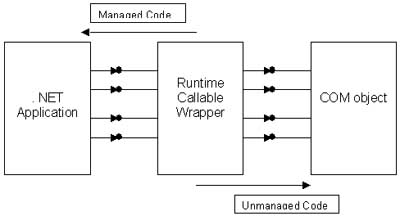
\includegraphics[scale=0.7]{Images/SchemaInterop.png} \\
	\textit{Source : Csharphelp \footnote{Csharphelp : \url{http://www.csharphelp.com}}}
\end{center}

Donc bien qu'il soit possible d'utiliser d'autres langages de programmation, nous nous contenterons de d�velopper en C\# afin de ne pas rajouter un travail de conversion suppl�mentaire. D'autant plus que C\# poss�de une syntaxe proche de celle de Java, il nous sera donc plus ais� de nous y adapter. Ainsi, nous ne perdrons pas de temps sur l'aspect aprentissage d'une nouvelle syntaxe.

\section{Biblioth�ques utilis�es}

En plus du framework .NET 3.5, nous utiliserons la LibSL afin de communiquer avec Second Life. A priori, il ne nous est pas n�cessaire d'utiliser d'autres bilbioth�ques. 
Si jamais nous serions amen� � communiquer avec des bases de donn�es, nous pourrons le faire en utilisant LINQ qui est directement int�gr� au Framework .NET 3.5, ce qui nous permettrai de faire directement nos appels aux bases dans le code source en C\#.

 Linden Lab, les cr�ateurs de Second Life, on developp� un langage de script pour Second Life : \keyword{LSL} (Linden Scripting Language). Dans le cadre de ce projet, nous ne pourrons pas l'utiliser car, ce langage est pratique pour faire des petits scripts (taille max des fichier 16Ko), mais inadapt� � de plus gros projets et surtout les scripts ne s'appliquent pas aux avatars. 
\myquote{A script in Second Life is a set of instructions that can be placed inside any primitive object in the world, but not inside an avatar.}
{\LL \footnote{LSL : \url{http://wiki.secondlife.com/wiki/Help:Getting_started_with_LSL}}} 

% Planning pr�visionnel et effectif
\chapter{Plannings}
\section{Planning pr�visionnel}
Voici le planning �tabli le 4 f�vrier 2009, disponible dans sa version $GanttProject$ en annexes.
Sur cette source (projet.gan), vous pourrez voir les ressources associ�es � chaque t�ches.
Ci-dessous, un apper�u est disponible
\begin{landscape}
	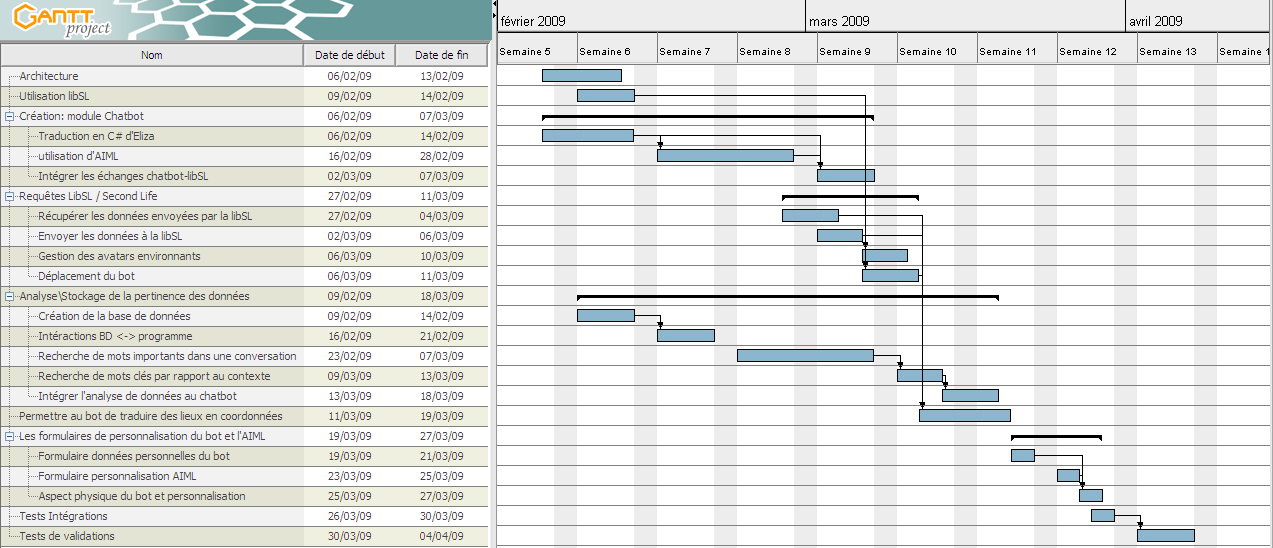
\includegraphics[scale=0.55]{Images/gantt.png}
\end{landscape}

% Architecture du logiciel, pour le moment la structure globale (seule, a venir : diagramme de classe, MCD, etc.)
% \chapter{Architecture logicielle}

\section{Architecture g�n�rale}
Voici la structure (simplifi�e) que nous allons mettre en place : 

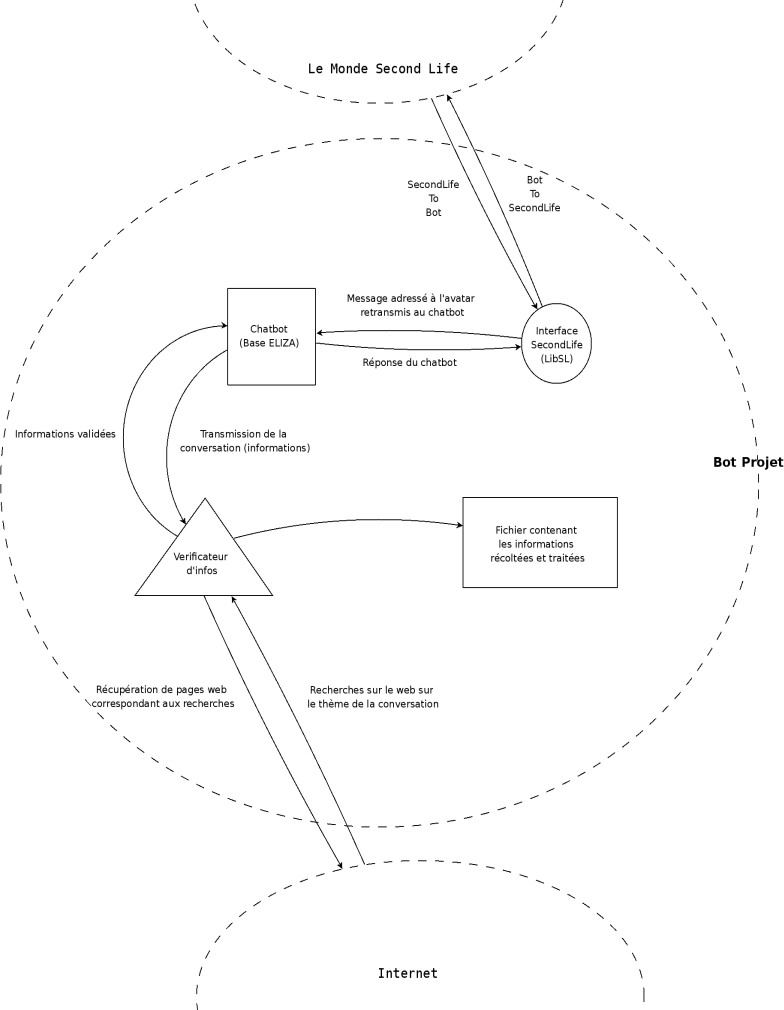
\includegraphics[scale=0.56]{Images/architectureGenerale.png} 
%--------------------

%-- Bibliographie ---
%\nocite*
\bibliographystyle{IEEEtranS}
\bibliography{Bibliographie/ia,Bibliographie/turing,Bibliographie/chatbot,Bibliographie/latex}
\textbf{\textit{Remarques}} : 
\begin{itemize}
	%\item Les r�f�rences non cit�es sont comment�es.
	\item Toutes les pages web ont �t� derni�rement consult�e le 12 janvier 2009
	\item Style de la bibliographie : Copyright (c) 2003 Michael Shell (IEEEtran)
\end{itemize}
%--------------------

%-- Index -----------
\printindex
%--------------------

\end{document}